\section{Reti Neurali}
\label{ANN}

Le reti neurali artificiali (ANN, \textit{artificial neural networks}), costituiscono i modelli di deep learning per eccellenza.

Una rete neurale può essere interpretata come un insieme di strati (\textbf{\textit{layer}}) composti ciascuno da un certo numero di unità computazionali, dette \textbf{neuroni}, che nell'insieme sono in grado di fornire una nuova rappresentazione dell'input, secondo il paradigma del \textit{representation learning}. Le funzioni sono composte a formare una catena di rappresentazioni sconosciute (per questo dette \textit{hidden layers}), nel senso che ciascun layer calcola una funzione dell'output del layer precedente: a partire da rappresentazioni più semplici, esse vengono raggruppate fino ad un livello di arbitraria complessità
\begin{equation*}
\mathcal{F}(\mathbf{x})=\mathbf{f}^{(d)}\underbrace{(\dots(\mathbf{h}^{(3)}(\mathbf{h}^{(2)}(\mathbf{h}^{(1)}(\mathbf{x})))))}_{\text{hidden layers}}
\end{equation*}
in cui
\begin{itemize}
\item $d$ è la profondità della rete, cioè il numero di layers che la compongono;
\item $\mathbf{h}^{(1)}$ è il primo (hidden) layer, $\mathbf{h}^{(2)}$ il secondo, e così via. Ciascuno di essi rappresenta una trasformazione parametrica in generale non lineare delle feature relative ad un input $\mathbf{x}$: ogni hidden layer $\mathbf{h}$ accetta un vettore in input $\mathbf{x}$, calcola una
trasformazione affine $\mathbf{z}=\mathbf{W}\mathbf{x}+\mathbf{b}$, quindi applica una funzione non lineare $g(\mathbf{z})$
elemento per elemento, detta \textbf{funzione di attivazione}. Si ottiene così:
\begin{align*}
\text{Layer 1: } & \hspace{8mm}\mathbf{h}^{(1)}=g^{(1)}\left(\mathbf{W}^{(1)}\mathbf{x}+\mathbf{b}^{(1)}\right)\\
\text{Layer 2: } & \hspace{8mm}\mathbf{h}^{(2)}=g^{(2)}\left(\mathbf{W}^{(2)}\mathbf{h}^{(1)}+\mathbf{b}^{(2)}\right)\\
\text{Layer 3: } & \hspace{8mm}\mathbf{h}^{(3)}=g^{(3)}\left(\mathbf{W}^{(3)}\mathbf{h}^{(2)}+\mathbf{b}^{(3)}\right)
\end{align*}
fino a giungere all'output layer:
\begin{align*}
\text{Layer d: } & \hspace{8mm}\mathbf{f}^{(d)}=g^{(d)}\left(\mathbf{W}^{(d)}\mathbf{h}^{(d-1)}+\mathbf{b}^{(d)}\right)
\end{align*}
\item $f^{(d)}$ è l'output layer, che ha il ruolo di fornire un'ultima trasformazione al fine di completare il task che la rete deve eseguire. Le scelte solitamente sono:
\begin{itemize}
\item Layer di output lineare: viene calcolata una ulteriore trasformazione affine, del tipo
\begin{equation*}
\mathbf{\widehat{y}}=\mathbf{W}\mathbf{h}^{(d-1)}+\mathbf{b}
\end{equation*}
\item Layer di output softmax: viene calcolata una trasformazione affine
\begin{equation*}
\mathbf{z}=\mathbf{W}\mathbf{h}^{(d-1)}+\mathbf{b}
\end{equation*}
e viene quindi applicata la \textbf{funzione softmax}
\begin{equation*}
\mathbf{\widehat{y}}=\text{softmax}(\mathbf{z})_i=\frac{e^{z_i}}{\sum\nolimits_{j}e^{z_j}}
\end{equation*}
Grazie alla funzione softmax, l'output $\mathbf{\widehat{y}}$ è la distribuzione di probabilità che $\mathbf{x}$ appartenga alla classe $i$:
\begin{equation*}
\widehat{y_i}=p(y=i|\mathbf{x})
\end{equation*}
\end{itemize}
\end{itemize}

La funzione di attivazione più utilizzata nell'ambito delle ANN è la seguente \textbf{ReLU} (Rectified Linear Unit), anche detta \textbf{rettificatore}:
\[\text{ReLU}(x)=x^{+}=\max(0,x)\]
Il rettificatore è la funzione di attivazione usata in tutte le reti neurali presentate in questo lavoro di tesi (par. \ref{alexnet}, \ref{googlenet}, \ref{resnet}).
Altre possibilità sono la sigmoide $g(x)=\sigma(x)$ oppure la tangente iperbolica $g(x)=\tanh(x)$.\\

\subsection{I neuroni}
\label{neuroni}
L'area di ricerca sulle ANN trae le sue origini dall'obiettivo degli scienziati di modellizzare matematicamente i sistemi neurali biologici che governano le facoltà intellettive del cervello umano.
È infatti possibile stabilire un confronto tra il neurone biologico e il "neurone" artificiale, definito nel precedente paragrafo, che ne costituisce una sua (semplicistica ma efficace) modellizzazione matematica.

Ogni neurone biologico (fig. \ref{fig:neuroneBiologico}) riceve segnali input dai suoi dendriti, e produce il segnale output lungo il suo (unico) assone. L'assone può eventualmente ramificarsi e connettersi via sinapsi ai dendriti di altri neuroni.

Nel modello computazionale (fig. \ref{fig:neuroneComputazionale}) del neurone, i segnali che viaggiono lungo gli assoni (ad es. gli $x_i$ in figura) sono pesati con un certo valore (i pesi $w_i$) che quantifica la "plasticità sinaptica"\footnote{La plasticità sinaptica è la capacità del sistema nervoso di modificare l'intensità delle relazioni interneuronali (sinapsi).} di quella sinapsi. I vari segnali pesati provenienti da tanti neuroni si sommano all'interno del corpo cellulare (assieme ad un bias $b$). Il risultato numerico è presentato all'assone di output passando per una funzione di attivazione ($f$ in figura), che rappresenta la frequenza di emissione del segnale da parte di un neurone biologico\footnote{È questa frequenza di emissione (più che il segnale in sé, che è assimilabile ad un impulso) a trasportare l'informazione.}.

\begin{figure}[h]
\centering
\begin{subfigure}[b]{0.48\textwidth}
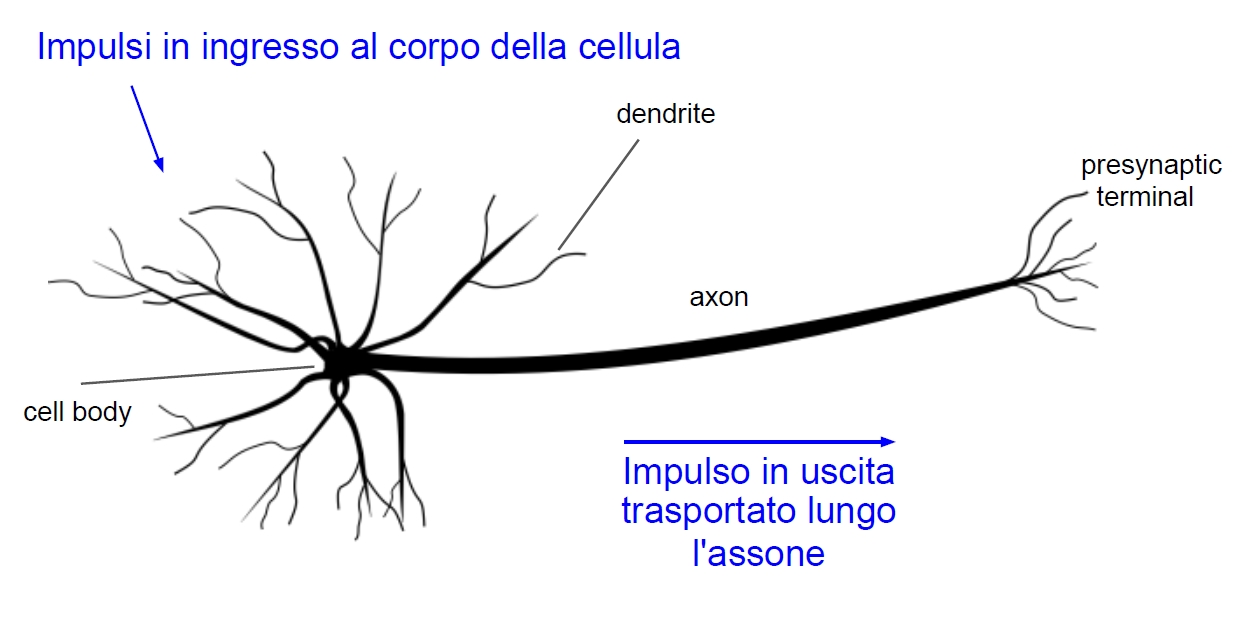
\includegraphics[width=\textwidth]{neuroneBiologico}
\caption{Disegno di un neurone biologico}
\label{fig:neuroneBiologico}
\end{subfigure}
\rulesep
\begin{subfigure}[b]{0.48\textwidth}
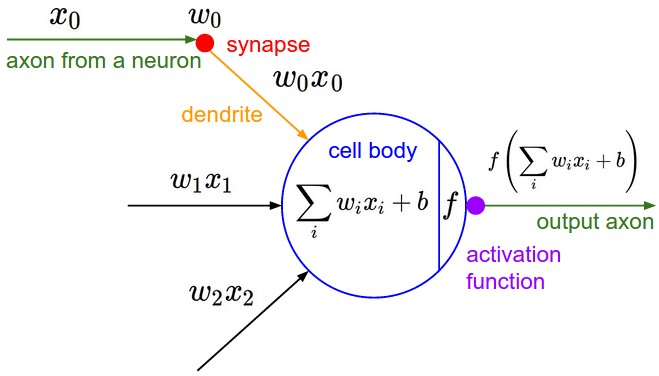
\includegraphics[width=\textwidth]{neuroneComputazionale}
\caption{Modello computazionale di un neurone}
\label{fig:neuroneComputazionale}
\end{subfigure}
\caption{Neuroni. Immagini tratte da: (a) \protect\url{https://thenounproject.com/term/neuron/214105/}, (b) \cite{cs231n}}
\label{fig:neurone}
\end{figure}

Ogni neurone si comporta quindi come la composizione di una funzione di attivazione $g$ con una funzione lineare (affine) $f(\mathbf{x}; \mathbf{w}, b)=\mathbf{w}^\top\mathbf{x}+b$; evidentemente, uno strato composto da neuroni si comporta come un classificatore lineare (par. \ref{classificatoreLineare}): ogni neurone di un certo strato $i$ aggiunge una riga alla matrice $\mathbf{W}^{(i)}$ dei pesi ed una al vettore $\mathbf{b}^{(i)}$ dei bias, associati a quello strato.\\

\subsection{Architettura delle reti neurali artificiali}
\label{architetturaANN}
Le reti neurali sono modellate come collezioni di neuroni connessi in un grafo aciclico diretto\footnote{in inglese \textit{direct acyclic graph} (DAG); particolare grafo orientato che non ha cicli diretti, ovvero comunque scegliamo un vertice del grafo non possiamo tornare ad esso percorrendo gli archi del grafo.}, organizzati in strati distinti.

Le architetture più "standard" delle reti neurali sono costituite da uno strato di input, uno o più \textbf{strati completamente connessi} (\textit{fully connected (FC) layer}) nei quali ciascun neurone è connesso a tutti i neuroni dello strato precedente e non esistono connessioni tra i neuroni dello stesso strato, ed infine uno strato di output. La fig. \ref{fig:esempioANN} mostra un esempio di rete neurale con soli layer FC.

\begin{figure}[h]
\centering
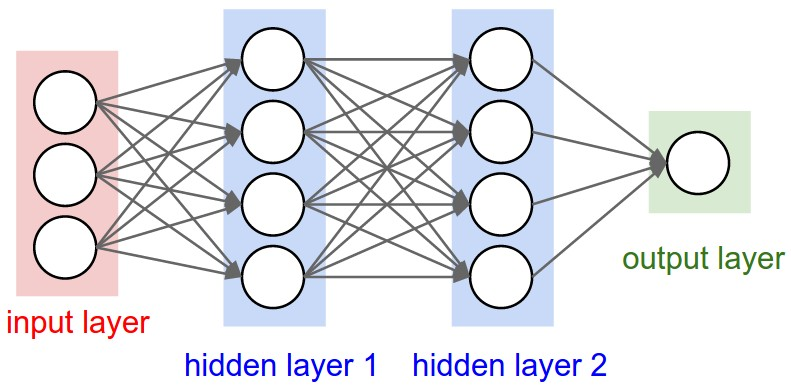
\includegraphics[width=0.7\textwidth]{esempioANN}
\caption{Una rete neurale con 3 strati (convenzionalmente non si conta quello di input) di cui due nascosti (\textit{hidden layers}) con 4 neuroni ciascuno e uno di output con un solo neurone.}
\label{fig:esempioANN}
\end{figure}

I valori reali assunti dai neuroni sono chiamati \textbf{attivazioni} dei neuroni.
Nei problemi di classificazione delle immagini (par. \ref{objectRecognition}), lo strato di input contiene neuroni in numero esattamente uguale a $hwc$, essendo le immagini accettate in input dalla rete di risoluzione $w\times h$ e con $c$ canali di colore. Ogni neurone contiene uno dei tre valori scalari che compongono un pixel. I neuroni dello strato di output sono in numero uguale a $|Y|$, il numero di categorie di oggetti che si possono classificare.

Spesso i neuroni dell'output layer non adoperano una funzione di attivazione (possiamo immaginare che usino la funzione identità). Nel caso di reti che svolgono un task di classificazione di immagini, come nel nostro caso, i valori delle attivazioni dei neuroni di output sono immessi nella funzione softmax per calcolare la distribuzione di probabilità da attribuire ad ogni classe di oggetti.

Le dimensioni di una rete neurale possono essere misurate con diverse metriche, tra cui il numero di neuroni o, più comunemente, il numero di parametri addestrabili. Ad esempio, la rete rappresentata in fig. \ref{fig:esempioANN} ha $4+4+1=9$ neuroni e quindi $3\times 4 + 4\times 4 + 4\times 1 = 32$ pesi e $4+4+1$ bias, per un totale di 41 parametri addestrabili.

Una rete neurale con strati completamente connessi può rappresentare una famiglia di funzioni (vettoriali di variabile vettoriale) parametrizzati dai pesi della rete.
È stato dimostrato \cite{approximation} che una rete neurale feedforward con un layer di output lineare e
almeno un hidden layer che abbia una funzione di attivazione tra quelle elencate in
precedenza può approssimare una qualsiasi funzione continua su un insieme chiuso e limitato di
$\R^{n}$ con un errore arbitrario.
Questo teorema fornisce una giustificazione teorica molto generica del funzionamento
delle reti neurali, ma non specifica nessun dettaglio riguardante l’architettura da utilizzare (es. numero di layer FC e numero di neuroni in ciascuno di essi)
per poter ottenere un errore di approssimazione desiderato. Le scelte riguardanti il
numero di layer, il numero di pesi per ciascun layer, il tipo di connettività tra i neuroni,
le funzioni di attivazione, il layer di output, ecc. derivano quasi sempre da risultati
sperimentali piuttosto che teorici.

Tutti i parametri della rete che non sono addestrabili ma che sono invece scelti arbitrariamente dal progettista (es. numero di layer della rete, input size, numero di neuroni in ogni layer, ecc.) si chiamano \textbf{iperparametri} della rete (\textit{hyperparameters}). Il loro valore ottimale non può essere trovato matematicamente (o meglio, spesso risulterebbe computazionalmente difficile farlo) ma possono essere scelti con un processo \textit{trial and error}.

\section{Reti neurali convoluzionali}
\label{CNN}
Una rete neurale si dice \textbf{convoluzionale} (\textit{convolutional}) se, in almeno uno dei layers, è utilizzata un'operazione di convoluzione al posto della consueta moltiplicazione tra matrici.

Grazie alla natura dell'operazione di convoluzione (par. \ref{convoluzione}), le reti neurali convoluzionali si sono rivelate particolarmente adatte al riconoscimento di pattern sia all'interno di segnali monodimensionali come audio o testo sia all'interno di segnali bidimensionali come le immagini. Questo è il motivo principale per cui sono state adoperate nell'ambito del task di classificazione binaria di immagini oggetto del presente lavoro (par. \ref{esperimentoTL}).
Per il resto del presente lavoro, ci riferiremo a CNN che lavorano esclusivamente su immagini e che nel suo strato finale utilizza la funzione softmax per calcolare la distribuzione di probabilità associata ad ogni classe dello spazio delle classi.

Una rete neurale convoluzionale è costituita da uno stack di layers, mostrato in fig. \ref{fig:convnet}: in input c'è un'immagine e in output c'è un vettore contenente la distribuzione di probabilità relativa alle categorie di oggetti classificabili.\\

L'architettura di una CNN può comporsi di strati di tipologie diverse\footnote{Va comunque notato che esistono numerosi altri strati che non sono presentati in questa sede. Alcuni di questi sono descritti nei paragrafi sulle tre CNN usate negli esperimenti, a cui pertanto si rimanda. Per una descrizione accurata di molti altri tipi di layer si rimanda a \url{https://code.google.com/archive/p/cuda-convnet/wikis/LayerParams.wiki}}

\begin{itemize}
	\item Input: generalmente un'immagine di dimensioni contenute (es. $224\times 224$). (par. \ref{INPUT})
	\item \textit{Convolutional layer} (CONV): vengono eseguiti diversi filtraggi sull'input, in maniera indipendente l'uno dall'altro, cioè un certo numero di convoluzioni con lo stesso dato in input ma con diversi kernel. (par. \ref{CONV}). Viene prodotto un set di \textit{feature map}.
	\item \textit{Activation layer} (detto anche \textit{ detector stage}): ciascun neurone dello strato precedente è passato ad una funzione di attivazione, tipicamente la ReLU. (par. \ref{RELU})
	\item \textit{Pooling layer} (POOL): viene eseguito un sottocampionamento dell'immagine attraverso una statistica riassuntiva delle regioni. (par. \ref{POOL})
	\item \textit{Fully-Connected layer} (FC): già descritti nella trattazione sulle reti neurali classiche; nell'ambito delle CNN sono finalizzati ad effettuare la classificazione vera e propria a partire dalle \textit{feature} estratte dai livelli convoluzionali precedenti. (par. \ref{FC})
	\item \textit{Softmax layer}: applica la funzione di attivazione softmax alla fine della rete, per calcolare la distribuzione di probabilità delle classi da predire. (par. \ref{SOFTMAX}
\end{itemize}

L'architettura di una CNN può prevedere una concatenazione di layer in serie (si parla in quest caso di \textit{series networks}, es. AlexNet par. \ref{alexnet}) ma anche una serie di modifiche che portano certi layer a funzionare in parallelo tra loro (ad es. il modulo \textit{inception} di GoogLeNet, par. \ref{inception}) o che comunque alterano il flusso lineare dell'informazione attraverso la rete mediante diramazioni (ad es. le \textit{skip connections} in ResNet, par. \ref{residualBlock}).

In questo modo, una rete CNN associa l'immagine in ingresso alla distribuzione di probabilità associata alle categorie classificabili.

Si noti che alcuni livelli contengono parametri e altri no. In particolare, i livelli Convolutional e Fully-Connected eseguono trasformazioni che sono funzione non solo delle attivazioni nel volume di input, ma anche dei parametri (i pesi e i bias dei neuroni). Invece, gli strati di attivazione e pooling implementeranno una funzione fissa, senza parametri addestrabili. I parametri degli strati CONV e FC vengono appresi in fase di addestramento attraverso l'applicazione dell'algoritmo di ottimizzazione \textit{stochastic gradient descent}, in modo che la distribuzione calcolati all'ultimo livello siano coerenti con le etichette del \textit{training set} per ogni immagine.

\begin{figure}[h]
	\centering
	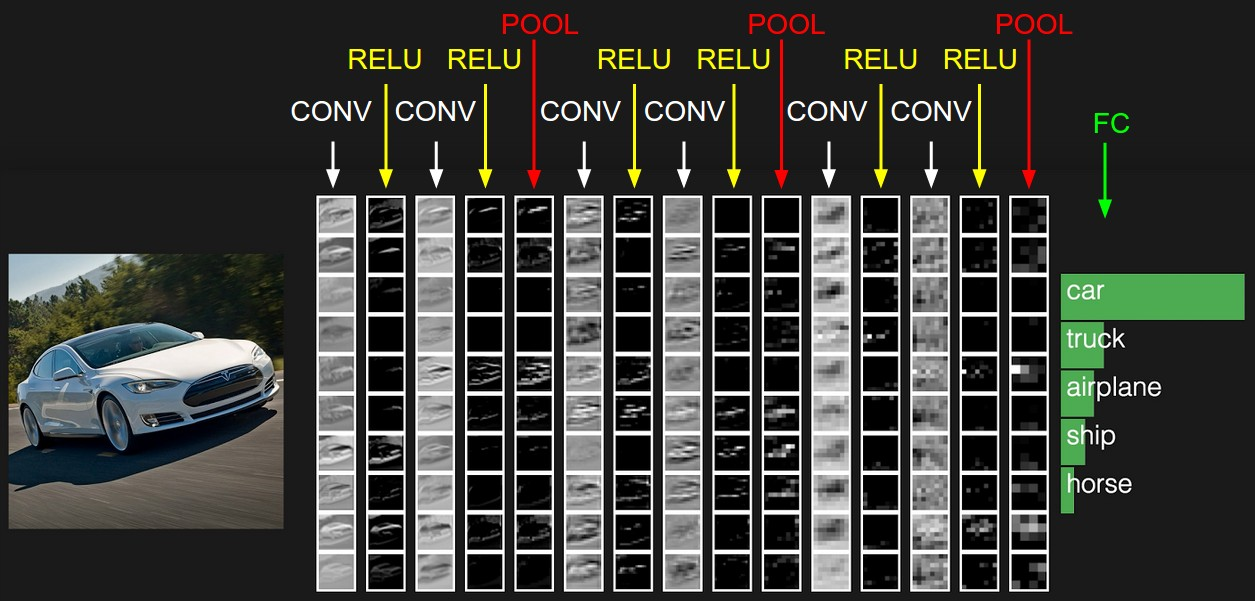
\includegraphics[width=0.7\linewidth]{convnet}
	\caption[Esempio di rete CNN]{Le attivazioni di un esempio di architettura ConvNet. Il volume iniziale memorizza i pixel dell'immagine in input (a sinistra) e l'ultimo volume memorizza la probabilità per ogni classe (a destra). Ogni volume di attivazioni lungo il percorso di elaborazione è mostrato come una colonna, in cui ogni immagine è una mappa bidimensionale di attivazione (vd. par. \ref{CONV}).}
	\label{fig:convnet}
\end{figure}

\subsection*{Volumi di attivazioni}
Come detto, le reti neurali convoluzionali ricevono in input delle immagini. Questo rende possibile un più "sensato" ed intuitivo arrangiamento dei neuroni nei vari layer. I neuroni sono infatti arrangiati in \textbf{volumi tridimensionali di attivazioni}. Così come le immagini hanno pixel arrangiati lungo la lunghezza, l'altezza e i canali di colore (profondità) dell'immagine, i neuroni di un certo strato possono essere arrangiati spazialmente lungo le stesse tre dimensioni. Allora si può dire che la rete opera una serie di trasformazioni che portano da un volume di attivazioni iniziale (quello determinato dall'immagine $w\times h\times 3$) ad uno finale: lo strato $i$-esimo trasforma il volume di attivazioni $i-1$-esimo nel volume $i$-esimo per mezzo di una funzione differenziabile.

Si veda la fig. \ref{fig:volume}. Al variare dell'indice $d$ del volume, che indica la terza dimensione del volume (la profondità, o \textit{volume depth}), si può univocamente identificare una sezione bidimensionale del volume, che chiameremo \textbf{mappa di attivazioni} (\textit{activation map}, anche detta \textit{depth slice}). In figura, ogni mappa di attivazioni è una griglia che contiene $a\times b$ neuroni.

\begin{figure}[h!]
\centering
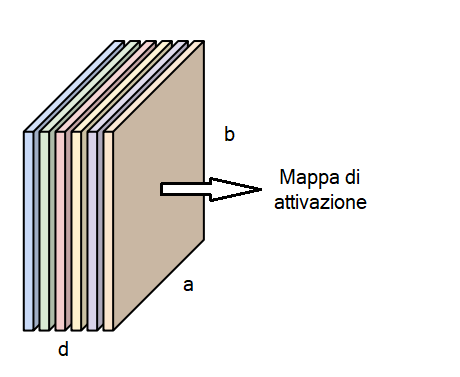
\includegraphics[width=0.4\textwidth]{volume}
\caption{Volume di attivazioni $a\times b\times d$}
\label{fig:volume}
\end{figure}


Si descrivono nel seguito con maggiore dettaglio i singoli layer, con le relative tecniche di implementazione in Matlab, utilizzate nel presente lavoro (par. \ref{esperimentoTL}).
Ogni tipo di layer esiste in Matlab come un tipo di dato complesso a se stante, ciascuno con la propria funzionalità.

In Matlab è possibile definire l'architettura di una CNN in due modi diversi:
\begin{enumerate}
\item Le reti i cui layer sono tutti "in serie" tra loros (es. AlexNet, par. \ref{alexnet}) sono rappresentate da un oggetto di tipo \verb|SeriesNetwork|, il quale contiene come campo un array di tipo \verb|Layer| che contiene (in ordine) gli strati della rete.
\item Le reti che hanno in generale un grafo aciclico diretto ma non in serie (es. GoogLeNet, par. \ref{googlenet}, ResNet-18 e 50, par. \ref{resnet}) sono rappresentate da un oggetto di tipo \verb|DAGNetwork|, il quale oltre al campo di tipo \verb|Layer| sopra citato contiene anche un altro campo di tipo \verb|table| di dimensioni $p\times 2$, dove $p$ è il numero di connessioni da stabilire tra i layer e le due colonne specificano rispettivamente il layer di partenza e quello di arrivo di ciascuna connessione.
\end{enumerate}

Entrambi questi oggetti possono essere passati come argomento della funzione \verb|trainNetwork| al fine di addestrare la rete.

\subsection{Input Layer}
\label{INPUT}
Rappresenta il layer di input alla rete per immagini 2D.
\begin{verbatim}
layer = imageInputLayer(inputSize,'Property',Value)
\end{verbatim}
\begin{itemize}
	\item \verb|inputSize| 
	
	Dimensione delle immagini in input, specificata come un vettore riga di 3 interi \verb|[h w c]|, con \verb|hxw| dimensione dell'immagine e \verb|c| numero di canali. Nel caso di immagini RGB, \verb|c| deve essere pari a 3.
	
	\item \verb|'Normalization', 'zero-centered'| oppure \verb|'none'|
	
	Specifica la trasformazione dei dati applicata in questo layer. Di default, viene applicata una centratura dei dati intorno allo zero, sottraendo l'immagine media del training set da ogni immagine di input. L'immagine media viene calcolata automaticamente a tempo di training dalla funzione \verb|trainNetwork|. In alternativa è possibile specificare esplicitamente l'immagine media da usare come parametro \verb|'AverageImage'| 
\end{itemize}

\subsection{Convolution Layer}
\label{CONV}
Il layer di convoluzione è il "cuore" delle reti neurali convoluzionali, in cui vengono effettuate importanti operazioni di filtraggio. Per ogni finestra dell'input, viene eseguita un'operazione di convoluzione (tridimensionale) tra il volume di attivazione $a\times b\times c$ e un kernel $h\times k\times c$, e per ogni mappa di attivazione ottenuta si aggiunge ai neuroni di quella mappa un termine di bias (vettore di bias $1\times 1\times c$) (fig. \ref{fig:cr}).

\begin{figure}[h]
	\centering
	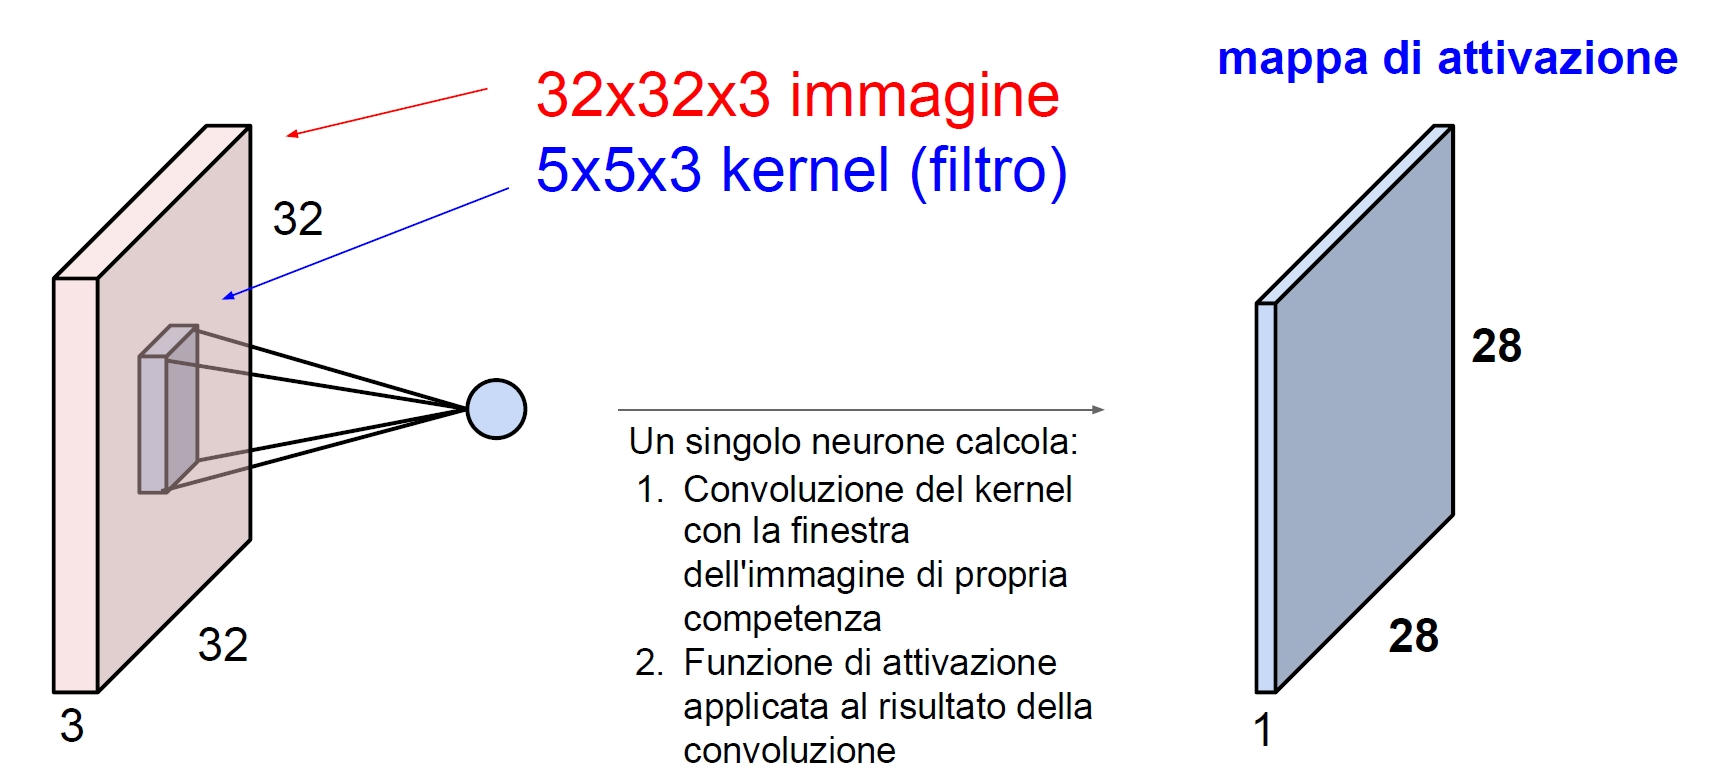
\includegraphics[width=0.7\linewidth]{CR}
	\caption[Convolution layer in una rete neurale convoluzionale]{Esempio di computazione di un neurone attraverso un layer di convoluzione e di attivazione. Utilizzando una convoluzione valida con stride pari a 1 e senza input padding, la convoluzione di un'immagine $32\times32\times3$ con un filtro $5\times5\times3$ produce una matrice $28\times28\times1$, cui viene applicata la funzione d'attivazione scelta per ottenere una activation map. Tutti i $28\times28$ neuroni impiegati per il calcolo di ogni singolo elemento che compone la mappa di attivazione utilizzano lo stesso filtro, cioè un kernel con gli stessi parametri (\textbf{parameter sharing})}
	\label{fig:cr}
\end{figure}

In Matlab, la creazione del layer avviene attraverso la funzione \texttt{\justify{convolution2dLayer}}:

\begin{verbatim}
layer = convolution2dLayer(filterSize,numFilters,'Property',Value)
\end{verbatim}

Gli argomenti sono:

\begin{itemize}
	\item \verb|filterSize|
	
	Dimensione del kernel, specificato come un intero \verb|F| per ottenere un filtro quadrato \verb|F x F|. Se si vogliono utilizzare dimensioni differenti (filtro in generale rettangolare) è possibile specificare un vettore \verb|[h w]|.
	
	\item \verb|numFilters|
	
	Numero dei filtri, specificato come un intero positivo \verb|K|. Questo parametro corrisponde al numero di neuroni nel layer di convoluzione che sono connessi alla stessa regione dell'input. Il volume di output avrà esattamente \verb|K| livelli di profondità (cioè \verb|K| mappe di attivazioni). (fig. \ref{fig:ca})
\end{itemize}

\begin{figure}[h]
	\centering
	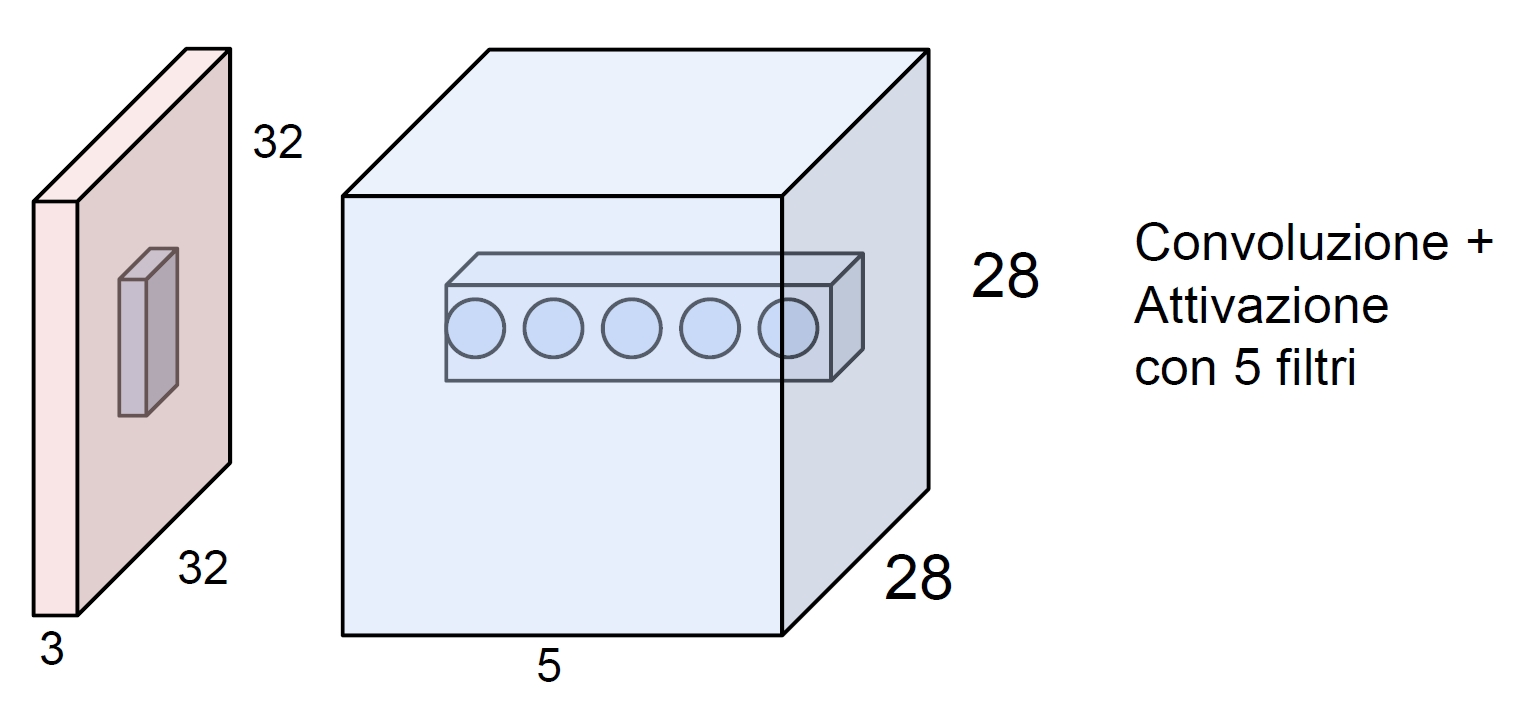
\includegraphics[width=0.7\linewidth]{CA}
	\caption[Output di un Convolution Layer]{I 5 neuroni mostrati applicano un diverso filtro (un kernel con diversi parametri) alla stessa regione spaziale dell'immagine in input, in maniera indipendente l'uno dall'altro.}
	\label{fig:ca}
\end{figure}

Gli eventuali parametri che possono essere specificati sono:

\begin{itemize}
	\item \verb|'Stride', S|
	
	Parametro che regola lo scorrimento della finestra del filtro sull'input. Se si specifica un intero positivo \verb|S|, gli scorrimenti della finestra sono caratterizzati da una traslazione di \verb|S| pixel in orizzontale e di \verb|S| pixel in verticale. Se si vogliono utilizzare traslazioni differenti rispetto alle due dimensioni è possibile specificare un vettore \verb|[h w]|.
	
	\item \verb|'DilationFactor', L|
	
	Fattore che specifica una convoluzione "dilatata". Se si specifica un intero positivo \verb|L| maggiore di 1, è come se il filtro venisse ampliato inserendo \verb|L-1| zeri tra ogni elemento. Il risultato è quello di ampliare la dimensione del campo ricettivo (\textit{receptive field}) rispetto all'input. Se si vuole utilizzare una dilatazione differente rispetto alle due dimensioni è possibile specificare un vettore \verb|[h w]|. (fig. \ref{fig:dilation})
	
\begin{figure}[h]
	\centering
	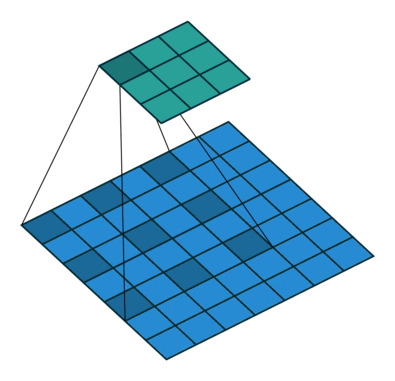
\includegraphics[width=0.3\linewidth]{dilation}
	\caption{Dilation di fattore L=2}
	\label{fig:dilation}
\end{figure}
	
	\item \verb|'PaddingSize', [t b l r]|
	
	Dimensione del padding da applicare all'input, specificata come un vettore di quattro interi positivi. Indicano rispettivamente il numero di righe nulle da aggiungere in alto (top) e in basso (bottom) e il numero di colonne nulle da aggiungere a sinistra (left) e a destra (right). Di default, il padding è nullo.
	
	\begin{figure}[h]
	\centering
	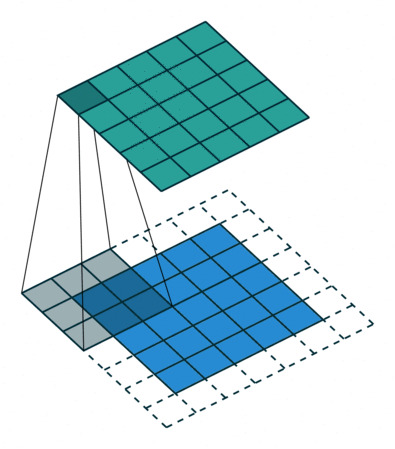
\includegraphics[width=0.3\linewidth]{padding}
	\caption{Padding con t=b=l=r=1}
	\label{fig:padding}
\end{figure}
	
	\item \verb|'PaddingMode', 'manual'| oppure \verb|'same'|
	
	Questa proprietà è utile se si vuole preservare la dimensione dell'input attraverso un layer di convoluzione. Specificando il valore \verb|'same'|, infatti, viene calcolato automaticamente il valore della dimensione del padding adatto a perseguire tale scopo. Per un filtro quadrato di dimensione \verb|F|, ad esempio, è necessario applicare un padding uniforme \verb|[P P P P]| con \verb|P = (F-1)/2|.
	
	\item \verb|'NumChannels','auto'| oppure \verb|n|
	
	Numero di canali (livelli di profondità) per ciascun filtro. Di default, questo parametro è sempre uguale alla profondità del tensore di input al livello di convoluzione
	
	\begin{figure}[h]
		\centering
		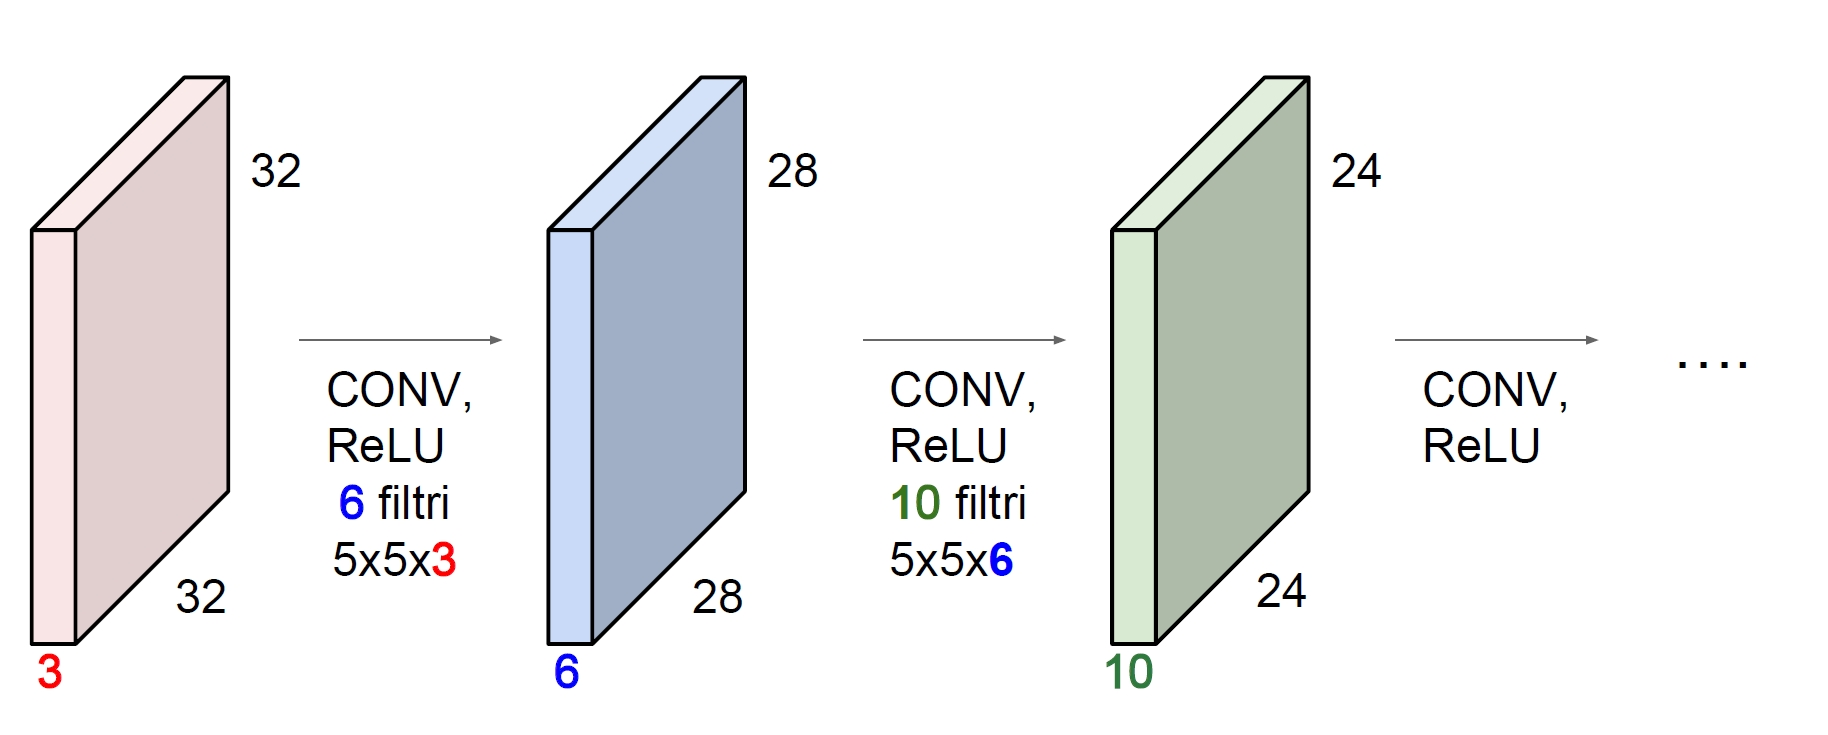
\includegraphics[width=0.7\linewidth]{channels}
		\caption[Profondità dei filtri attraverso una CNN]{La figura mostra come la profondità dei filtri di ogni livello di convoluzione debba essere equivalente alla profondità dell'input del rispettivo livello}
		\label{fig:channels}
	\end{figure}

	\item \verb|'Weights', W|
	
	\verb|Weights| è l'array contenente i pesi del layer, ovvero i parametri che definiscono le convoluzioni e che vengono appresi dalla rete durante la fase di addestramento. Se l'input al layer è di profondità \verb|D_i|, il kernel è di dimensione \verb|F| e il numero di filtri è pari a \verb|K|, allora \verb|Weights| sarà un array \verb|4-D single| di dimensione \verb|F|$ \times $\verb|F|$ \times $\verb|D_i|$ \times $\verb|K|, in cui la quarta dimensione indicizza ogni filtro. Specificando questa proprietà, è possibile inizializzare i pesi con un vettore a propria scelta \verb|W|.
	
	\item \verb|'Bias', B|
	
	\verb|Bias| è l'array contenente i parametri di bias, ovvero i parametri che vengono sommati al risultato delle convoluzioni, anch'essi appresi dalla rete durante la fase di addestramento. Se \verb|K| è il numero di filtri applicato nel layer, allora \verb|Bias| sarà un array \verb|3-D single| di dimensioni \verb|1|$\times$\verb|1|$\times$\verb|K|
	
	\item \verb+'WeightsInitializer','glorot'|'he'| 'narrow-normal'|'zeros'|'ones'+
	
	Funzione utilizzata per l'inizializzazione dei pesi in \verb|Weights|. Le alternative sono:
	
	\begin{itemize}
		\item \verb|'glorot'|: generatore pseudocasuale utilizzato di default, con una distribuzione uniforme a media nulla e varianza \verb|2/(numIn+numOut)|, con \verb|numIn=F|$\times$\verb|F|$\times$\verb|D_i| e \verb|numOut=F|$\times$\verb|F|$\times$\verb|K|
		
		\item \verb|'he'|: generatore pseudocasuale di una distribuzione uniforme a media nulla e varianza \verb|2/numIn|, con \verb|numIn=F|$\times$\verb|F|$\times$\verb|D_i|
		
		\item \verb|'narrow-normal'|: generatore pseudocasuale di una distribuzione uniforme a media nulla e varianza 0.01
		
		\item \verb|'zeros'|: inizializza con tutti zeri
		
		\item \verb|'ones'|: inizializza con tutti 1
		
		\item \verb|function handle|: utilizza una funzione \textit{custom}
		
	\end{itemize}
	
	\item \verb+'BiasInitializer','zeros'|'narrow-normal'|'ones'|function handle+
	
\end{itemize}

Learning rate (locale) e regolarizzazione:

\begin{itemize}
	\item \verb|'WeightLearnRateFactor',alfa|
	
	Fattore da moltiplicare per il parametro learning rate globale relativo all'apprendimento dei pesi, di default pari a 1
	
	\item \verb|'BiasLearnRateFactor',beta|
	
	Fattore da moltiplicare per il parametro learning rate globale relativo all'apprendimento dei bias, di default pari a 1
	
	\item \verb|'WeightL2Factor',lambda1|
	
	Fattore da moltiplicare per il parametro globale di regolarizzazione L2 relativo all'apprendimento dei pesi, di default pari a 1
	
	\item \verb|'BiasL2Factor',lambda2|
	
	Fattore da moltiplicare per il parametro globale di regolarizzazione L2 relativo all'apprendimento dei bias, di default pari a 1
	
\end{itemize}

\subsection{Activation layer}
\label{RELU}
Il layer di attivazione è implementato, nel caso di funzione ReLU (l'unica che utilizzeremo in questo lavoro di tesi), mediante \verb|relulayer|.

\subsection{Pooling layer}
\label{POOL}
Una funzione di pooling opera un sottocampionamento sull'immagine, come mostrato in figura \ref{fig:pooling}.  Ogni regione di una certa dimensione dell'immagine in input (es. $4\times4$) viene ridotta ad un unico pixel, il cui valore è calcolato tramite una statistica riassuntiva della regione di partenza (es. max, media, norma L2).
\begin{figure}[h!]
\centering
\begin{subfigure}[b]{0.48\textwidth}
\centering
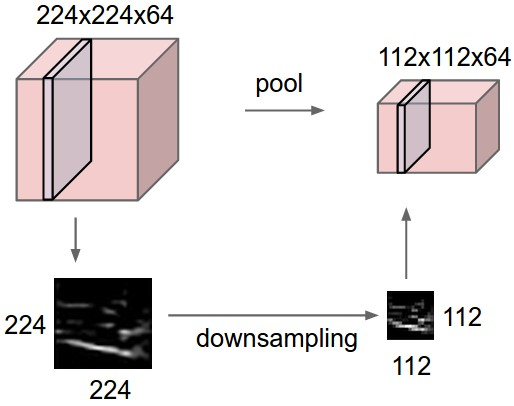
\includegraphics[width=\textwidth]{pool}
\caption{}
\end{subfigure}

\begin{subfigure}[b]{0.48\textwidth}
\centering
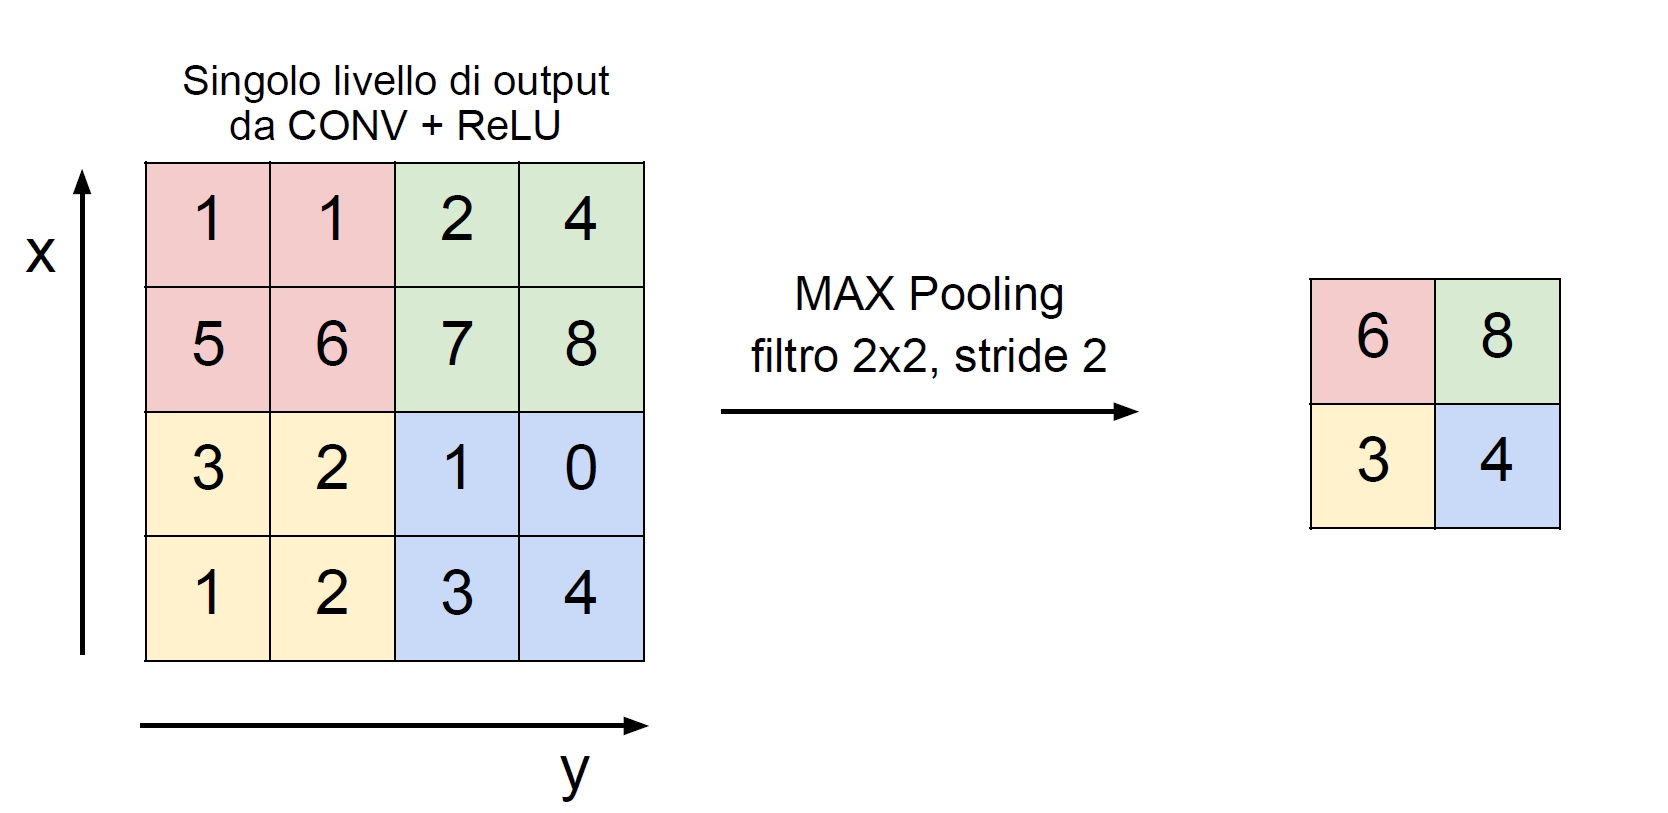
\includegraphics[width=\linewidth]{pooling}
\caption{}
\end{subfigure}
\caption{Operazione di pooling: (a) effetto di downsampling; (b) calcolo del max pooling}
\label{fig:pooling}
\end{figure}

L'utilità del pooling è quella di ridurre progressivamente la dimensione spaziale dei volumi che "scorrono" nell'architettura, per ridurre la quantità di parametri e di calcolo nella rete. Tipicamente, l'operazione è eseguita mediante un filtro di dimensioni $2\times 2$ (o anche $3\times 3$) applicato con uno stride di 2. Il risultato è quello di ridurre del 75\% il numero delle attivazioni propagate. Ogni operazione di max pooling richiederebbe in questo caso un massimo di 4 numeri (regione $2\times 2$). La dimensione della profondità del tensore di attivazione rimane invariata.\\

La funzione utilizzata per la sua creazione è \verb|maxPooling2dLayer|

\begin{verbatim}
layer = maxPooling2dLayer(poolSize,'Property',Value)
\end{verbatim}
\begin{itemize}
	\item \verb|PoolSize|
	
	Dimensione delle regioni di pooling, specificata come un intero positivo \verb|F|, in caso di finestra quadrata oppure un vettore di due interi positivi \verb|[h w]|, con \verb|h| altezza e \verb|w| larghezza della finestra
\end{itemize}
Le proprietà di questo layer sono del tutto analoghe a quelle del  \verb|convolution2dLayer| per ciò che riguarda il comportamento ai bordi e le modalità di traslazione della finestra. Si possono perciò parimenti specificare le proprietà \verb|'Stride'|, \verb|'PaddingSize'| e \verb|'PaddingMode'|.

\subsection{Fully Connected Layer}
\label{FC}
Moltiplica l'input per un tensore di pesi (di dimensioni pari a quelle del volume in input al layer) e aggiunge un vettore bias (di dimensione pari al numero di neuroni del layer FC). Ciascun neurone è connesso con tutti i neuroni del layer precedente. Un esempio numerico è mostrato in fig. \ref{fig:fc}.\\

I layer fully connected si implementano in Matlab con:
\begin{verbatim}
layer = fullyConnectedLayer(outputSize,'Property',Value)
\end{verbatim}

dove:

\begin{itemize}
	\item \verb|outputSize|
	
	Dimensione di uscita del fully connected layer, specificato come un numero intero positivo \verb|C|. Nel caso in cui il layer sia posto alla fine della rete (layer FC di classificazione, che fornisce valori alla funzione softmax finale), \verb|C| deve essere uguale al numero delle classi $|Y|$ da individuare all'interno del dataset.
\end{itemize}

\begin{figure}[h]
	\centering
	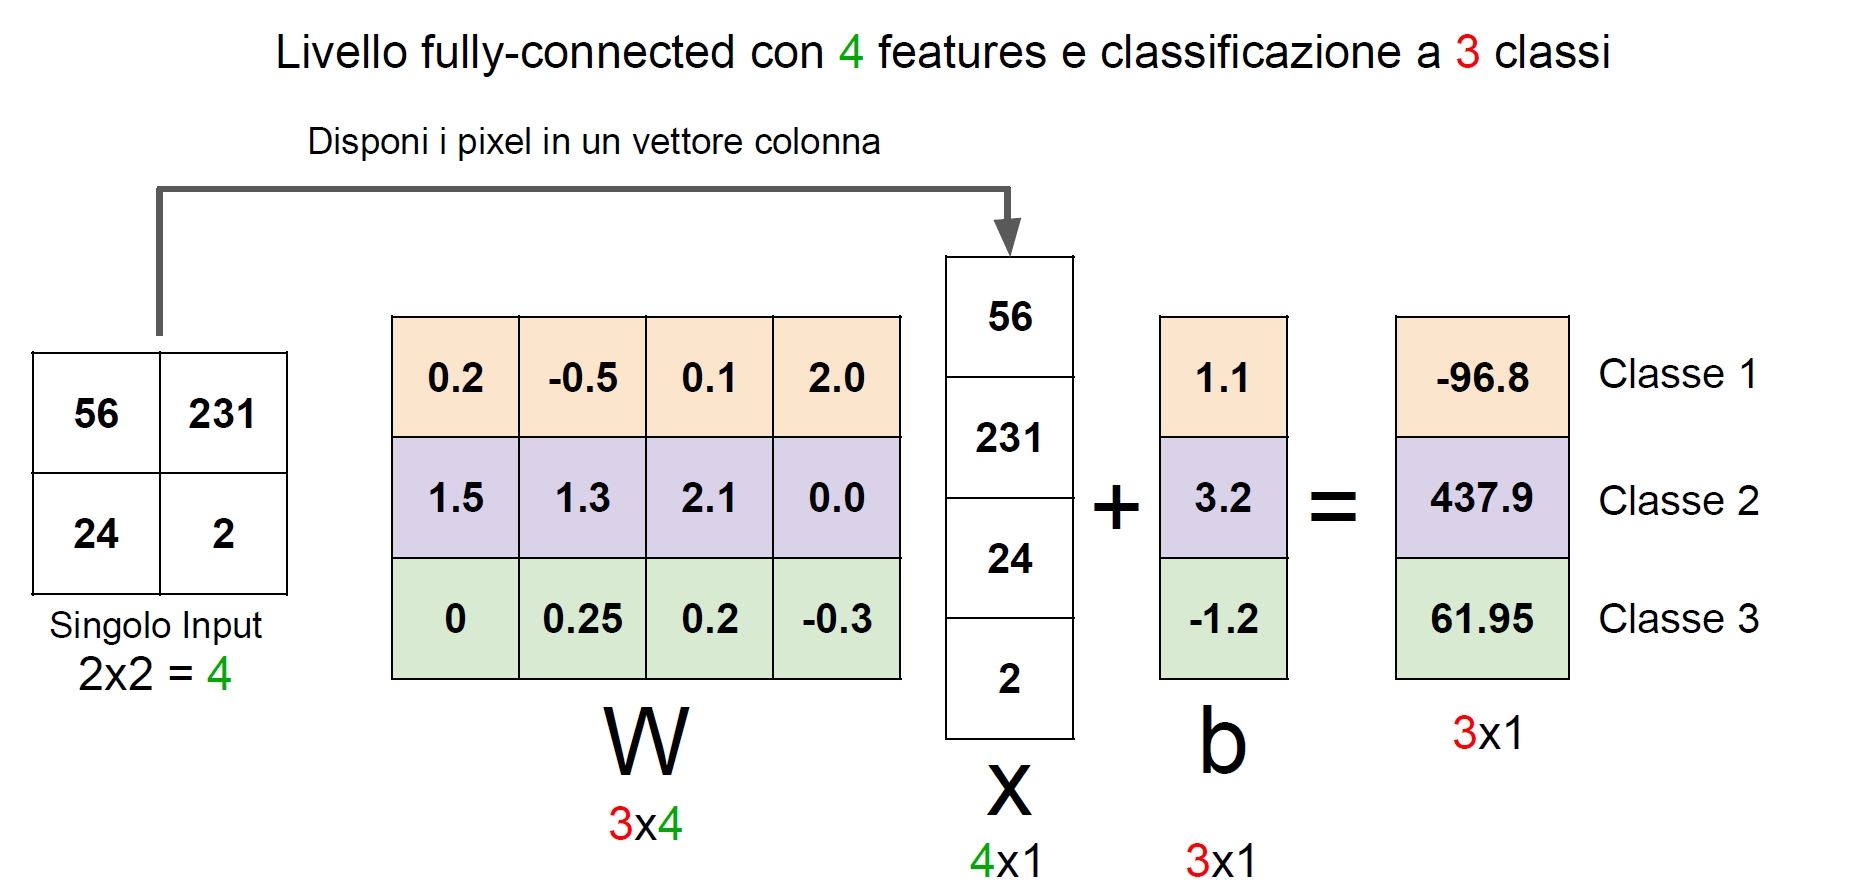
\includegraphics[width=0.7\textwidth]{fc}
	\caption{Esempio numerico di livello fully connected con un singolo input}
	\label{fig:fc}
\end{figure}

\subsection{Softmax layer}
\label{SOFTMAX}
La funzione di attivazione finale softmax, inserita in coda all'ultimo fully connected layer, è implementata mediante \verb|softmaxLayer|.



\section{Image preprocessing e augmentation}
\label{augmentation}

La tecnica dell'\textbf{\textit{image preprocessing}} consiste in generale nel trasformare le immagini (esempi) di un dataset per mezzo di operazioni sulle sue feature. Tipicamente, queste operazioni sono applicate alle immagini di un training set prima che ci si serva di esso per addestrare un classificatore, ma possono essere applicate anche sui test set.
Le trasformazioni possono includere centraggio delle feature, normalizzazione, traslazioni, rotazioni, riflessioni, scalatura, e così via.

In generale, ci sono due motivi per cui si vuole effettuare il preprocessing di un training set:

\begin{itemize}
\item Rendere le immagini più semplici da elaborare da parte di una rete neurale. Ad esempio, il centraggio e la normalizzazione delle feature possono essere utili ad evitare eventuali problemi di overflow e stabilità numerica nelle operazioni eseguite dalla rete.

\item Migliorare la capacità di generalizzazione del modello. Nel caso dell'\textit{image classification}, le classi rispetto a cui il classificatore deve produrre un output sono infatti spesso invarianti rispetto ad un'ampia varietà di trasformazioni negli input, facilmente realizzabili. Operazioni geometriche come traslazioni, rotazioni, riflessioni, scalatura (già viste nel par. \ref{trasformazioni}) possono essere implementate come semplici operazioni sui pixel (trasformazioni affini) e si rivelano particolarmente utili (se eseguite in modo casuale ma accorto) per la riduzione dell'errore di generalizzazione della maggior parte di modelli di computer vision.
\end{itemize}

Tra le forme di preprocessing più comunemente utilizzate su un'immagine (esempio) $\mathbf{x}$ di un training set per assolvere al primo dei due obiettivi del preprocessamento delle immagini citiamo:

\begin{itemize}
\item \textbf{Sottrazione della media} (\textit{mean subtraction}), che consiste nel sottrarre ad ogni feature dell'esempio la media di tutte le feature. L'interpretazione geometrica di questa operazione è il centraggio delle feature attorno allo 0.

\item \textbf{Normalizzazione} dei pixel. Solitamente un'immagine a colori rappresentata come un tensore a 3 canali RGB ha ogni pixel rappresentato da un intero senza segno di 1 byte, quindi nel range $[0,255]$. Si può quindi fare in modo che tutti i pixel siano normalizzati in un range ragionevole, come $ [0,1] $ oppure $ [-1,1] $.
Un'ulteriore forma di normalizzazione è la divisione di ogni feature per la deviazione standard di tutte le feature (operazione che va applicata solo dopo il centraggio attorno allo 0 delle feature, con la sottrazione della media).
\end{itemize}

Il secondo obiettivo del preprocessamento è particolarmente critico nel caso in cui il training set a nostra disposizione è relativamente piccolo e poco eterogeneo (cioè con poca variabilità nelle immagini di una stessa classe). Spesso training set piccoli non sono sufficienti per addestrare la rete in maniera soddisfacente, rendendo il rischio di overfitting particolarmente concreto.

Al fine di aggirare questo problema si mette in campo una strategia di \textbf{\textit{image augmentation}}, una particolare forma di \textit{image preprocessing} che ha come scopo quello di ingrandire (\textit{augment}) il training set con nuovi esempi, generati in vario modo a partire da quelli del training set originale.

Le trasformazioni di \textit{augmentation} sono in genere scelte in maniera casuale (con una certa probabilità per ciascuna) per ogni esempio da "aumentare", da un set di operazioni specificato a priori da chi addestra la rete.

Tra le operazioni di \textit{image augmentation} più comuni citiamo:

\begin{itemize}
\item Estrarre da ogni esempio dei ritagli rettangolari da posizioni differenti.
\item Applicare trasformazioni geometriche affini, quali quelle descritte nel par. \ref{trasformazioni}.
\item Applicare distorsioni fotometriche e cromatiche di vario tipo.
\end{itemize}

Bisogna comunque osservare che per dataset grandi ed eterogenei solitamente si fanno poche operazioni di augmentation di questo tipo, poichè si lascia imparare al modello a quale tipo di fattori di variazione esso deve essere invariante.\\

In Matlab è possibile ottenere la versione aumentata di un dataset con un oggetto di tipo \verb|augmentedImageDatastore|. Esso consente di trasformare un dataset, definito in un oggetto \verb|imageDatastore| (vd. par. \ref{datastore}) con eventuali operazioni di preprocessing e augmentation specificate in un oggetto di tipo \verb|imageDataAugmenter|.
Un oggetto \verb|augmentedImageDatastore| può essere passato semplicemente come argomento della funzione \verb|trainNetwork| (vd. par. \ref{addestramento}), per essere utilizzato come \textit{training set} di una rete neurale. In tal caso, per ogni \textit{epoch} (quindi a \textit{runtime}), i dati di training vengono casualmente perturbati e ridimensionati all'input size della rete\footnote{Il ridimensionamento è necessario affinché tutte le immagini rispettino la dimensione di input della rete neurale, che è fisso.}, in modo che ciascuna \textbf{\textit{epoch}} (epoca), cioè un ciclo di addestramento sull'intero training set, usi un training set leggermente diverso. Il numero effettivo di immagini usate per ciascuna \textit{epoch} non cambia. Le immagini trasformate non vengono memorizzate. L'\verb|imageInputLayer| di una CNN normalizza le immagini ad ogni \textit{epoch}, sottraendo un'intensità media costante calcolata un'unica volta, subito dopo la augmentation relativa alla prima \textit{epoch}. In fig. \ref{fig:augmentationTraining} viene mostrato il processo di addestramento di una rete neurale adoperando un augmentedImageDatastore.\\

\begin{figure}[h]
\centering
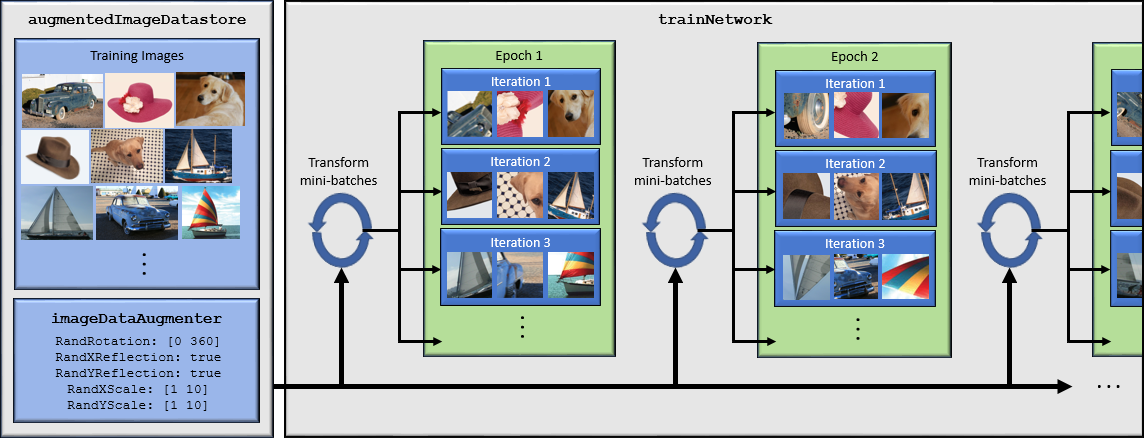
\includegraphics[width=0.9\textwidth]{augmentationTraining}
\caption{Processo di addestramento (mediante \textit{stochastic gradient descent} con dimensione del mini-batch = 3) in cui il training set è definito con un oggetto augmentedImageDatastore}
\label{fig:augmentationTraining}
\end{figure}

La creazione di un oggetto \verb|augmentedImageDatastore| avviene invocando la funzione

\begin{verbatim}
auimds = augmentedImageDatastore(outputSize,imds)
\end{verbatim}

Altri argomenti opzionali sono:

\begin{itemize}

	\item \verb|NumObservations|: numero totale di "osservazioni" nella collezione di immagini aumentate. Coincide con la lunghezza di ogni training \textit{epoch}, quindi coincide con l'omonima proprietà dell'oggetto \verb|trainingOptions| (vd. par. \ref{addestramento}) e può essere modificato solo di lì (proprietà READ-ONLY).
	
	\item \verb|Files|: oggetto \verb|cell array| contenente le directory delle immagini ereditate dall'oggetto \verb|imageDatastore| con cui è stato costruito)
	
	\item \verb|MiniBatchSize|: dimensione del mini-batch utilizzato durante l'addestramento dal metodo \textit{stochastic gradient descent} per il calcolo della funzione costo. Coincide con l'omonima proprietà dell'oggetto \verb|trainingOptions| e può essere modificato solo di lì (proprietà READ-ONLY).
	
	\item \verb|DataAugmentation|: oggetto di tipo \verb|imageDataAugmenter| che consente di definire trasformazioni di preprocessing da applicare alle immagini
	
	\item \verb|ColorPreprocessing|: eventuali conversioni \verb|'gray2rgb'| o \verb|'rgbtogray'| per fare in modo che tutte le immagini abbiano lo stesso numero di canali richieste dall'\verb|imageInputLayer| della rete neurale.
	
	\item \verb|OutputSize|: dimensione delle immagini di output, come vettore di due interi positivi. L'operazione di ridimensionamento è l'unica operazione di augmentation prevista di default, al fine di rendere le immagini compatibili con la dimensione di input specificata nell'\verb|imageInputLayer|
	
	\item \verb|OutputSizeMode|: metodo utilizzato per il ridimensionamento delle immagini
	
	\begin{itemize}
		\item \verb|'resize'|: le immagini vengono scalate utilizzando la interpolazione bilineare con antialiasing (operazione più veloce ma con risultati di qualità inferiore rispetto alla interpolazione bicubica utilizzata da \verb|imresize|. Evita distorsioni causate dalla interpolazione nearest-neighbor). Questa opzione è di default.
		\item \verb|'centercrop'|: viene effettuato un ritaglio al centro dell'immagine della dimensione specificata in \verb|OutputSize|
		\item \verb|'randcrop'|: viene effettuato un ritaglio in una posizione casuale dell'immagine della dimensione specificata in \verb|OutputSize|
	\end{itemize}
\end{itemize}

Se non è specificato come argomento un oggetto \verb|imageDataAugmenter|, l'unica operazione di preprocessing svolta è il ridimensionamento all'input size della rete.

La sintassi per creare un oggetto \verb|imageDataAugmenter| è:

\begin{verbatim}
aug = imageDataAugmenter('Property',Value,...)
\end{verbatim}

in cui è possibile definire le opzioni di \textit{image augmentation} esprimendo una o più coppie proprietà-valore. Tra le varie possibilità, citiamo solo quelle effettivamente utilizzate all'interno del presente lavoro:
\begin{itemize}
	\item \verb+'RandXReflection', true|false+ \newline\vspace{0.1mm}\verb+'RandYReflection', true|false+
	
	Ogni immagine subisce con una probabilità del 50\% una riflessione orizzontale (\verb|X|) oppure verticale (\verb|Y|)
	\item \verb|'RandRotation',[a b]|
	
	Applica una rotazione con un angolo, espresso in gradi, estratto da una distribuzione uniforme pseudocasuale nell'intervallo $[a,b]$
	\item \verb|'RandXTranslation',[a b]|\newline\vspace{0.1mm}\verb|'RandYTranslation',[a b]|
	
	Applica una traslazione orizzontale (\verb|X|) oppure verticale (\verb|Y|) all'immagine. L'entità della traslazione, misurata in pixel, è estratta da una distribuzione uniforme pseudocasuale nell'intervallo $[a,b]$
\end{itemize}

\section{Addestrare una rete neurale}
Per poter essere impiegata per risolvere un certo task, una rete neurale deve essere opportunamente addestrata. Addestrare una rete neurale significa individuare un set di valori per i parametri addestrabili della rete che le permettono di approssimare la funzione desiderata (cioè che le permettano di risolvere efficacemente il task).
Un addestramento efficace rende la rete capace di generalizzare in modo appropriato, cioè di dare risposte plausibili per input che non ha mai visto.\\

Riferendoci ad una rete che svolge un task di \textit{image classification} (ma si può facilmente estendere la spiegazione ad una ANN standard), l'addestramento della rete avviene in due diversi stadi: \textit{forward-pass} (propagazione in avanti) e \textit{backward-pass} (propagazione all'indietro).
\begin{itemize}
\item Nel \textit{forward-pass} a partire dalle immagini in input si calcolano di strato in strato tutti i volumi intermedi fino al volume finale, che permette la classificazione. Durante questa fase i valori dei parametri addestrabili sono tutti fissati.
\item Nel \textit{backward-pass} la risposta della rete (la distribuzione di probabilità della predizione) viene confrontata con l'uscita desiderata (la distribuzione di probabilità che assegna probabilità 1 alla effettiva classe di appartenenza dell'immagine e 0 alle rimanenti) ottenendo il segnale d'errore, calcolato per mezzo della funzione costo (par. \ref{loss}). L'errore calcolato è propagato nella direzione inversa rispetto a quella del \textit{forward-pass}. I parametri sono aggiornati ad ogni iterazione in modo da minimizzare la funzione costo, tramite un metodo di minimizzazione come la discesa stocastica del gradiente (par. \ref{SGD}), che calcola il gradiente della funzione costo rispetto ad ogni parametro con l'algoritmo di backpropagation (par. \ref{backpropagation}).
\end{itemize}

\subsection{Inizializzazione dei parametri}
\label{weights}
Prima di addestrare la rete, i parametri devono essere inizializzati con valori casuali, che saranno poi alterati durante il training.\\
Delle scelte comuni per i pesi sono:
\begin{itemize}
\item estrazione di un valore casuale della variabile aleatoria $\varepsilon \mathcal{X}$, dove $\varepsilon$ è piccolo (tipicamente 0.01) e $\mathcal{X}$ è la v.a. gaussiana standard (media nulla e varianza unitaria).
\item estrazione di un valore casuale della variabile aleatoria $\frac{\mathcal{X}}{\sqrt{n}}$, dove $\mathcal{X}$ è la v.a. gaussiana standard e $n$ è il numero di parametri associati al nodo a cui il parametro di cui si è estratta l'inizializzazione appartiene.
\item estrazione di un valore casuale della variabile aleatoria $\frac{\mathcal{X}}{\frac{2}{\sqrt{n}}}$, con le stesse variabili descritte al punto precedente
\end{itemize}

\subsection{Loss function}
\label{loss}
Abbiamo visto che una rete neurale per l'\textit{image classification} accetta in input un'immagine e restituisce un punteggio per ogni classe da predire, o equivalentemente una probabilità per ogni classe (calcolata dalla funzione di attivazione softmax). In fig. \ref{class_lin} si era visto che quel particolare classificatore lineare assegnava all'immagine di un gatto un punteggio molto alto alla classe 'cane' ed uno molto basso alla classe 'gatto', classificandola pertanto come 'cane'. Il set di parametri costituito da $\mathbf{W}$ e $\mathbf{b}$ non è molto buono. Per misurare l'entità dell'errore commesso dalla rete nella classificazione definiamo una \textbf{funzione costo} (\textbf{\textit{loss function}}) anche detta funzione obiettivo (\textit{objective}).

Tra le varie loss function che si possono adoperare, quella utilizzata nel presente lavoro è la \textbf{\textit{cross-entropy loss}}, che è quella tipica delle reti che sfruttano la funzione softmax per effettuare la predizione.
Dato un training set (eventualmente aumentato) $X$ contenente $|X|$ immagini $\mathbf{x}^{(i)}$ ($i=1,\dots,|X|$), ciascuna appartenente alla classe $i$-esima, uno spazio delle etichette $Y$ e una rete neurale che associa all'immagine $|Y|$ punteggi diversi $s_j$ per ciascuna classe $j$-esima ($j=1,\dots,|Y|$), si definisce cross-entropy loss relativa al training set $X$ la funzione
\[
L=\underbrace{\frac{1}{|X|}\sum_{i=1}^{|X|}L_i}_{\text{data loss}}+\underbrace{\lambda R(\mathcal{W})}_{\text{regularization loss}}
\]
dove
\begin{itemize}
\item \begin{align*}
L_i=-\log\left(\frac{e^{s_i}}{\sum\nolimits_{j}e^{s_j}}\right) & \text{ o equivalentemente} & L_i=-s_i+\log\left(\sum\nolimits_{j}e^{s_j}\right)
\end{align*}
è il contributo alla cross-entropy loss di un singolo esempio del dataset. Esso è tanto maggiore quanto più la rete si comporta "male" sull'esempio $\mathbf{x}^{(i)}$. Si noti che nella prima parentesi è utilizzata la funzione softmax($s_j$).

\item $\mathcal{W}$ è l'insieme di tutti i parametri addestrabili della rete.

\item $R(\mathcal{W})$, detto penalità di regolarizzazione, può essere scelto tra varie funzioni; quella che utilizzeremo in questo lavoro è la cosiddetta norma L2:
\[
R(\mathcal{W}) = \sum_l\sum_k W_{l,k}^2
\]
dove $W_{l,k}$ rappresenta la $k$-esima matrice di pesi (e bias, con il bias trick) nell'$l$-esimo layer della rete, e l'elevamento a potenza della matrice è da intendersi come la somma dei quadrati di tutti i suoi elementi. Esso è tanto maggiore quanto più i parametri addestrabili della rete si discostano da 0. Minimizzare il termine $\lambda R(\mathcal{W})$ significa allora avvicinare i parametri a 0, tanto più velocemente ad ogni iterazione quanto più $\lambda$ (iperparametro) è grande.
$\lambda R(\mathcal{W})$

\end{itemize}

È evidente che addestrare la rete significa allora risolvere un problema di ottimizzazione, che consiste nel minimizzare la loss function calcolata su tutto il training set. La minimizzazione può avvenire con il classico metodo del calcolo numerico della discesa del gradiente, visualizzato in fig. \ref{fig:gd}.

Nella pratica, tuttavia, pensare di calcolare la loss function su tutto il training set è impensabile se la cardinalità del training set è molto elevata. Allora, ad ogni iterazione dell'addestramento, si preferisce utilizzare una versione approssimata della loss function, calcolata su un sottoinsieme piccolo di esempi del training set. La minimizzazione della loss function avviene in questo caso con il metodo della discesa stocastica del gradiente (par. \ref{SGD} e fig. \ref{fig:sgd}).

\subsection{Stochastic gradient descent}
\label{SGD}
Si può immaginare il grafico della funzione $L$ come una "vallata multidimensionale", differenziabile ovunque\footnote{poiché composizione di funzioni differenziabili} e con numerosi minimi locali, uno (o alcuni) dei quali può essere un minimo globale, come mostrato in figura \ref{vallata} in 3 dimensioni, nel caso (non molto plausibile ma semplice da visualizzare) di rete con soli due parametri addestrabili.

\begin{figure}[h!]
\centering
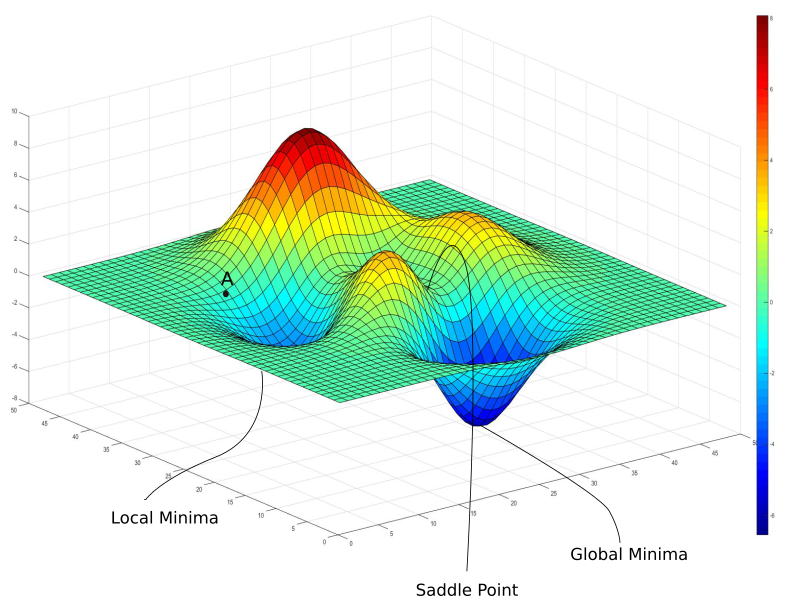
\includegraphics[width=0.8\textwidth]{vallata}
\caption{Grafico di una loss function con due sole variabili}
\label{vallata}
\end{figure}

Minimizzare la loss function significa individuare un\footnote{l'esistenza di un minimo globale non ne implica l'unicità: possono esserci più minimi locali di $L$ di uguale valore, che potrebbero anche essere minimi globali di $L$.} suo punto di minimo globale, partendo da un punto casuale e seguendo la direzione opposta a quella del \textbf{gradiente di $L(\mathcal{W})$} (la "discesa" verso il punto di minimo è cioè "guidata" dal gradiente di $L$). Il gradiente di $L(\mathcal{W})$ si indica con $\nabla L(\mathcal{W})$.

Il metodo della \textbf{discesa stocastica del gradiente} (\textit{stochastic gradient descent}, SGD), usato per minimizzare la loss function, prevede di calcolare $L$ non più sull'intero training set ma su un suo sottoinsieme detto \textbf{\textit{mini-batch}}, costituito da un numero ridotto di esempi (valori tipici sono 16, 32, 64, 128 o 256). La $L^{*}$ così ottenuta è ovviamente una approssimazione della $L$, tanto più buona quanto più il mini-batch è grande e "vario" (cioè quanto più gli esempi di ogni classe sono proporzionalmente presenti nel mini-batch). L'addestramento prevede allora che un'epoca di addestramento sia in realtà divisa in $\frac{|X|}{|\text{mini-batch}|}$ iterazioni per epoca, in ognuna delle quali si presenta alla rete un mini-batch, si calcola la relativa $L^{*(i)}(\mathcal{W})$, si calcola il gradiente $\nabla L^{*(i)}(\mathcal{W})$ e si effettua un "salto" $\Delta \mathcal{W}^{(i)}$ da un punto (calcolato all'iterazione precedente in base alla $L^{*(i-1)}$) ad un altro del dominio di $L^{*(i)}$. Il salto $\Delta \mathcal{W}^{(i)}$ è un vettore di $|\mathcal{W}|$ componenti, ciascuna delle quali rappresenta l'aggiornamento $\Delta w^{(i)}$ del parametro $w^{(i)}$ ed è dato da (supponendo $w^{(i)}$ appartenente all'$l$-esimo layer):
\[
\Delta w^{(i)}=-\text{glr}\times \text{llr}_l\times \frac{\partial L^{*(i)}}{\partial w^{(i)}}
\]
dove con glr = \textbf{learning rate globale} e $\text{llr}_l$ = \textbf{learning rate locale} dell'$l$-esimo layer. Questi sono iperparametri che caratterizzano rispettivamente la rete e i layer addestrabili della rete.\\

Il metodo della discesa del gradiente classico e quello stocastico sono confrontati in figura \ref{fig:gdConfronto}.

\begin{figure}[h!]
\centering
\begin{subfigure}[b]{0.48\textwidth}
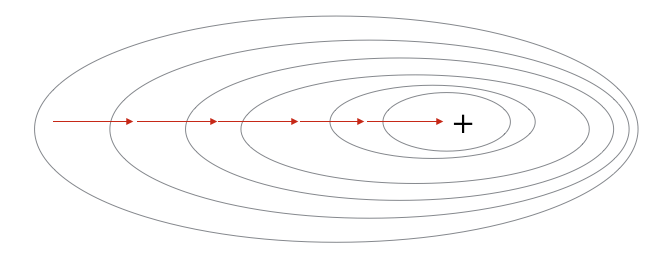
\includegraphics[width=\textwidth]{gd}
\caption{Gradient descent}
\label{fig:gd}
\end{subfigure}
\begin{subfigure}[b]{0.48\textwidth}
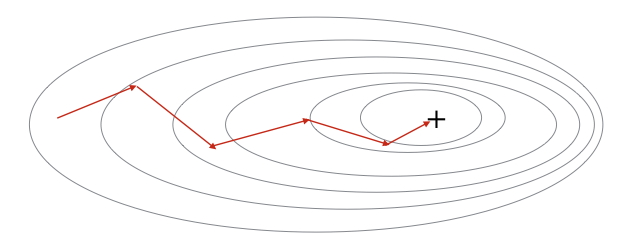
\includegraphics[width=\textwidth]{sgd}
\caption{Stochastic gradient descent}
\label{fig:sgd}
\end{subfigure}
\caption{}
\label{fig:gdConfronto}
\end{figure}

\noindent Alcune importanti osservazioni:

\begin{itemize}

\item La discesa del gradiente converge verso uno dei punti di minimo locale di $L$, non necessariamente in un punto di minimo globale come invece si desidera. Si può dimostrare che la regolarizzazione dei parametri aiuta ad appiattire il grafico di $L$, rendendo i minimi locali e il minimo globale tanto più vicini quanto più i parametri sono "regolarizzati". In queste condizioni, non è un problema il particolare punto di minimo locale in cui la rete converge alla fine dell'addestramento.

\item Nel metodo SGD, ad ogni iterazione il grafico della loss function varia. Se il mini-batch è, come discusso in precedenza, abbastanza grande e vario, le approssimazioni $L^{*(i)}$ sono abbastanza simili tra loro e a $L$ stessa, quindi in questa ipotesi possiamo affermare con buona approssimazione che il punto di minimo verso cui il metodo SGD sta convergendo rimane inalterato ad ogni iterazione.

\item La scelta del learning rate globale e di quelli locali è fondamentale: un learning rate più grande porta ad una convergenza più veloce del metodo SGD verso un punto di minimo locale di $L^{*(i)}$, ma si corre il rischio che dopo molte iterazioni il metodo non sia ancora del tutto "sceso" in uno dei minimi. Infatti per convergere ad un punto di minimo quando si è nelle sue vicinanze c'è bisogno di fare salti di piccola ampiezza verso di esso, a causa della forma a "campana rovesciata" del grafico della funzione attorno ai suoi minimi. Al contrario, un learning rate più piccolo comporta una certa lentezza nella convergenza ma assicura, dopo un sufficiente numero di iterazioni, una loss function più vicina ad un suo minimo. Si può allora mediare tra i due bisogni prevedendo una strategia di \textbf{annealing} (decadimento) del learning rate nel tempo. Ci sono tre tipi comuni di annealing:

\begin{itemize}

\item Step decay: si riduce il learning rate di un certo fattore dopo un certo numero di epoche (ad esempio si dimezza il learning rate ogni 5 epoche)

\item Exponential decay: si riduce il learning rate seguendo la funzione $\text{lr}=\text{lr}_0 e^{-kt}$, dove $\text{lr}_0$ è il learning rate iniziale, $k$ è un iperparametro che regola la velocità di decadimento, $t$ è il "tempo" trascorso (di solito è il numero di iterazioni trascorse o, più comunemente, il numero di epoche trascorse).

\item $1/t$ decay: si riduce il learning rate seguendo la funzione $\text{lr}=\text{lr}_0 /(1+kt)$; le variabili che compaiono hanno lo stesso significato del punto precedente.

\end{itemize}

\end{itemize}
 
\subsubsection{SGD with momentum}
Una variante frequentemente adoperata del metodo SGD è il metodo di \textbf{discesa stocastica del gradiente con momento} (\textit{stochastic gradient descent with momentum}, SGDM).
Il \textbf{momento} è un termine dipendente dalle iterazioni precedenti, che viene sommato al gradiente nel tentativo di regolarizzare il movimento nello spazio dei parametri.
La differenza con l'SGD classico consiste nel salto da compiere nel dominio di $L^{*(i)}$: ad ogni iterazione il salto $\Delta \mathcal{W}^{(i)}$ ha componente (lungo la dimensione del generico parametro $w^{(i)}$ appartenente all'$l$-esimo layer):
\[
\Delta w^{(i)}=-\text{glr}\times \text{llr}_l\times \frac{\partial L^{*(i)}}{\partial w^{(i)}}+\underbrace{\mu\times\Delta w^{(i-1)}}_{\text{momento}}
\]

L'effetto del momento è simile a quello che in fisica ha la quantità di moto (in inglese \textit{momentum}) nello spostamento di un oggetto: così come una forza che sposta un oggetto in una direzione gli fa acquistare velocità (quindi quantità di moto) in quella direzione, l'opposto del gradiente della loss function fa acquistare "velocità" nello spostamento verso il punto di minimo di $L^{*(i)}$, cosicché se il gradiente ha una certa stabilità nella sua direzione per più iterazioni, nell'iterazione successiva il salto avrà una componente lungo quella direzione, a prescindere dal particolare comportamento del gradiente in quella iterazione, "per inerzia".

Questo metodo introduce un ulteriore iperparametro $\mu$ (compreso tra 0 e 1) per controllare l'effetto del momento, ovvero l'importanza dell'iterazione passata: più è grande $\mu$ e più il termine momento assume importanza nell'aggiornamento $\Delta \mathcal{W}^{(i)}$. Un valore empirico per tale parametro è solitamente fissato intorno a 0.9.\\

Il metodo SGDM è visualizzato in fig. \ref{fig:sgdm}

\begin{figure}[h!]
\centering
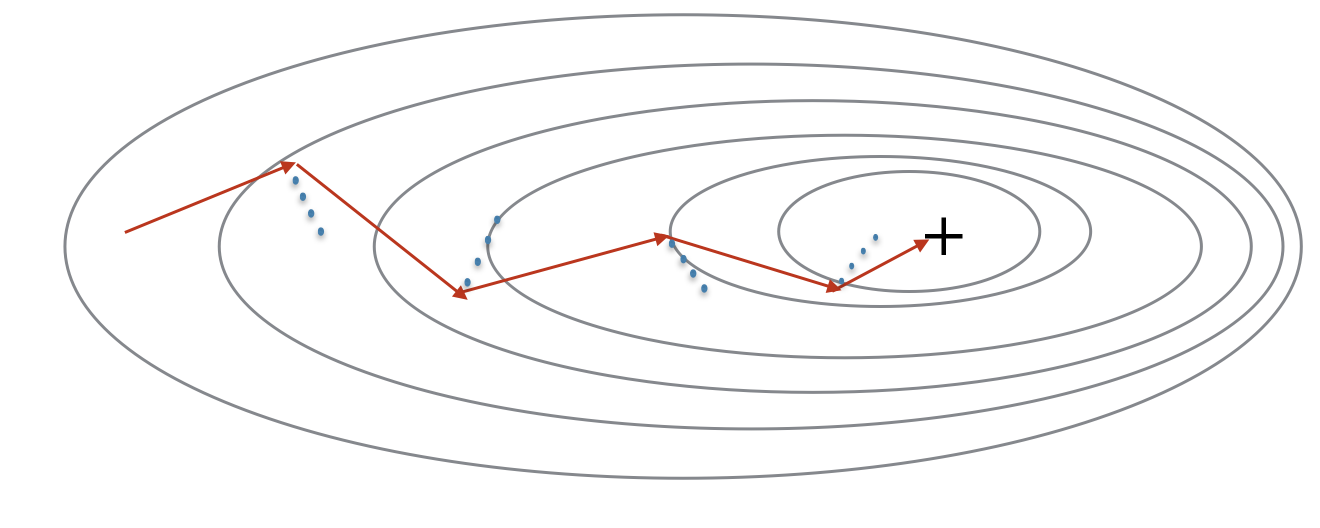
\includegraphics[width=0.5\textwidth]{sgdm}
\caption{Stochastic gradient descent with momentum}
\label{fig:sgdm}
\end{figure}

\subsection{Backpropagation}
\label{backpropagation}
Il calcolo del gradiente della loss function, nell'ambito del metodo SGD e SGDM, avviene analiticamente con il metodo di \textbf{\textit{(error) backpropogation}} (retropropagazione dell'errore). Questo metodo ricorre all'uso ricorsivo della "regola della catena" della derivazione per calcolare le derivate parziali $\frac{\partial L^{*(i)}}{\partial w^{(i)}}$; il calcolo si basa solamente sui valori di output della rete (i punteggi finali per ogni classe). Ad esempio, per una rete neurale standard (con soli strati completamente connessi seguiti ciascuno da una funzione di attivazione $g$) l'algoritmo di backpropagation calcola:
\[
\frac{\partial L^{*(i)}}{\partial w_{ij}^k}=g'(a_j^k)o_i^{k-1}\sum_{l=1}^{r^{k+1}}w_{jl}^{k+1}\delta_l^{k+1}
\]
dove $w_{ij}^k$ è il peso del collegamento tra il neurone $j$ del layer $k$ e il neurone $i$ del layer $k-1$, $a_i^k$ è il valore dell'attivazione del neurone i del layer $k$ prima dell'applicazione di $g$, $o_i^k$ è l'output del neurone $i$ nel layer $k$, $r_k$ è il numero di nodi nel layer $k$, $\delta_j^k=\frac{\partial L^{*(i)}}{\partial a_j^k}$.\\

Per maggiori approfondimenti sull'algoritmo di backpropagation, si rimanda ad esempio a \cite{dlbook}.

\subsection{Scomparsa ed esplosione del gradiente}
\label{vanishingGradient}
Il problema della \textbf{scomparsa del gradiente} (\textit{vanishing gradient problem}) è un fenomeno che crea difficoltà nell'addestramento delle reti neurali profonde tramite SGD/SGDM e backpropagation.

Una delle principali cause è la presenza di funzioni di attivazione non lineari classiche, come la tangente iperbolica o la sigmoide, che hanno gradiente a valori nell'intervallo $(0,1)$.
Poiché nell'algoritmo di retropropagazione i gradienti ai vari livelli vengono moltiplicati tramite la regola della catena, il prodotto di $n$ numeri in $(0,1)$ decresce esponenzialmente rispetto alla profondità $n$ della rete, rendendo quasi nullo l'aggiornamento dei parametri negli strati più bassi della rete.

Inoltre, valori grandi (in valore assoluto) passati alle funzioni di attivazione citate si trovano in zone del dominio delle funzioni dette "di saturazione", in cui la derivata è prossima allo 0. Ciò acuisce il problema numerico sopracitato.\\

Quando invece il gradiente delle funzioni di attivazione può assumere valori elevati, un problema analogo che può manifestarsi è quello dell'\textbf{esplosione del gradiente} (\textit{exploding gradient problem}).\\

Come si vedrà nei paragrafi dedicati alla descrizione delle reti neurali convoluzionali utilizzate negli esperimenti, il problema della scomparsa e dell'esplosione del gradiente viene risolto tipicamente usando funzioni di attivazioni ReLU e, dall'avvento di ResNet, le cosiddette \textit{skip connections} (par. \ref{residualBlock}).

\section{Transfer Learning}
\label{transferLearning}
Nella pratica, poche persone costruiscono e addestrano reti neurali da zero con inizializzazione casuale dei parametri (\textit{from scratch}) per risolvere un task, poiché è relativamente raro disporre di un training set di dimensioni adeguate. Un'alternativa è riutilizzare una rete addestrata su un dataset molto grande (es. ImageNet, par. \ref{imagenet}) e ri-addestrandola per risolvere il task di interesse, con dovuti accorgimenti che saranno spiegati nel seguito.
Questa tecnica si chiama \textbf{\textit{transfer learning}}.

Per esempio, possiamo riutilizzare una rete che è stata addestrata a classificare gatti e cani ri-addestrandola per riconoscere invece formiche e vespe. Se il dataset utilizzato nel task originale è più grande di quello disponibile per il secondo task, il transfer learning è in grado di aumentare significativamente la capacità di generalizzazione (e quindi le performance) del classificatore.
Il motivo per cui il transfer learning funziona è che molte categorie condividono alcune caratteristiche di basso livello come bordi, forme geometriche, cambi nell'intensità dell'illuminazione ecc \cite{howtransferable}. In generale, quindi, il transfer learning è una forma di representation learning usata con successo quando esistono concetti comuni ad un basso livello di astrazione tra le categorie del primo e del secondo task.

L'applicazione del transfer learning è schematizzata in fig. \ref{fig:transferLearning}

\begin{figure}[h!]
\centering
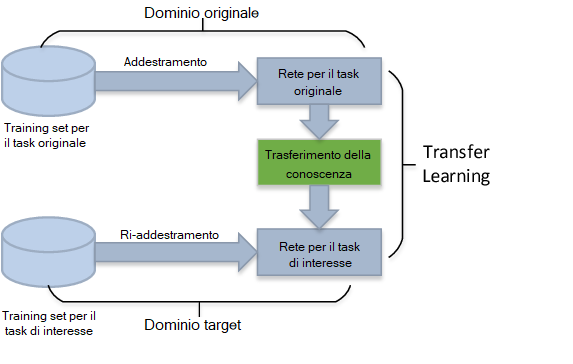
\includegraphics[width=0.75\textwidth]{transferLearning}
\caption{Schema di applicazione del transfer learning}
\label{fig:transferLearning}
\end{figure}

Il metodo del transfer learning per l'addestramento di un modello di classificazione consiste nei seguenti passi:
\begin{enumerate}
\item Selezione di una rete pre-addestrata

Al giorno d'oggi è estremamente facile reperire reti pre-addestrate: molte istituzioni di ricerca rendono pubblici modelli addestrati su dataset ampi e complessi (es. ImageNet), che possono essere riutilizzati per la tecnica del transfer learning.

\item (Opzionale) Azzerare i learning rate dei layer addestrabili più bassi

Questo passaggio ha l'obiettivo di "congelare" l'apprendimento dei layer che rappresentano le feature di livello più basso delle immagini, cioè inibire modifiche ai parametri addestrabili di quei layer. Generalmente, più piccolo è il training set a disposizione per il task di interesse e più layer iniziali andrebbero congelati; con pochi dati, infatti, c'è il rischio di overfitting della rete, problema aggirabile limitando la capacità di rappresentazione del modello che si vuole addestrare.

\item (Opzionale) Aumentare i learning rate dei layer addestrabili finali

Questo passaggio ha l'obiettivo di velocizzare l'apprendimento dei layer che rappresentano le feature di livello più alto delle immagini, al fine di migliorare la capacità della rete di mettere insieme le feature estratte nei livelli intermedi per effettuare la predizione.

\item Rimpiazzare il layer di classificazione finale

Si rimpiazza questo layer per cambiare le classi da predire: non più le classi del task originale (es. le mille classi di ImageNet) ma quelle del task di interesse (es. 'Pinna' e 'No Pinna').

\item Addestrare la rete.

La rete pre-addestrata, opzionalmente modificata a livello dei suoi learning rate locali, è usata come punto di partenza per il nuovo addestramento, che la porterà ad adattarsi al task di interesse.

\item Misurare le prestazioni del modello "trasferito" con un test set.

\end{enumerate}

Il transfer learning è utilizzato nel presente lavoro per adattare quattro modelli pre-addestrati al task di classificazione delle pinne dorsali dei cetacei (cap. \ref{esperimenti}).

\section{Ensemble learning}
\label{ensemble}
Al fine di migliorare l'accuratezza della classificazione, spesso si ricorre ad una strategia conosciuta come \textbf{apprendimento ensemble} (\textit{ensemble learning}). L'idea chiave è quella di creare un insieme (\textit{ensemble}) di classificatori di immagini, ciascuno dei quali è chiamato a "votare" circa l'esito della predizione; a seconda dello "schema di consenso" (\textit{consensus scheme}) scelto per l'ensemble, cioè a seconda di quanto peso assume ciascun voto nella classificazione finale, l'output complessivo sarà la classe che avrà ricevuto "democraticamente" il maggior consenso. La fig. \ref{fig:ensembleSchema} mostra lo schema di funzionamento di un classificatore ensemble.
\vspace{3mm}

\begin{figure}[h]
\centering
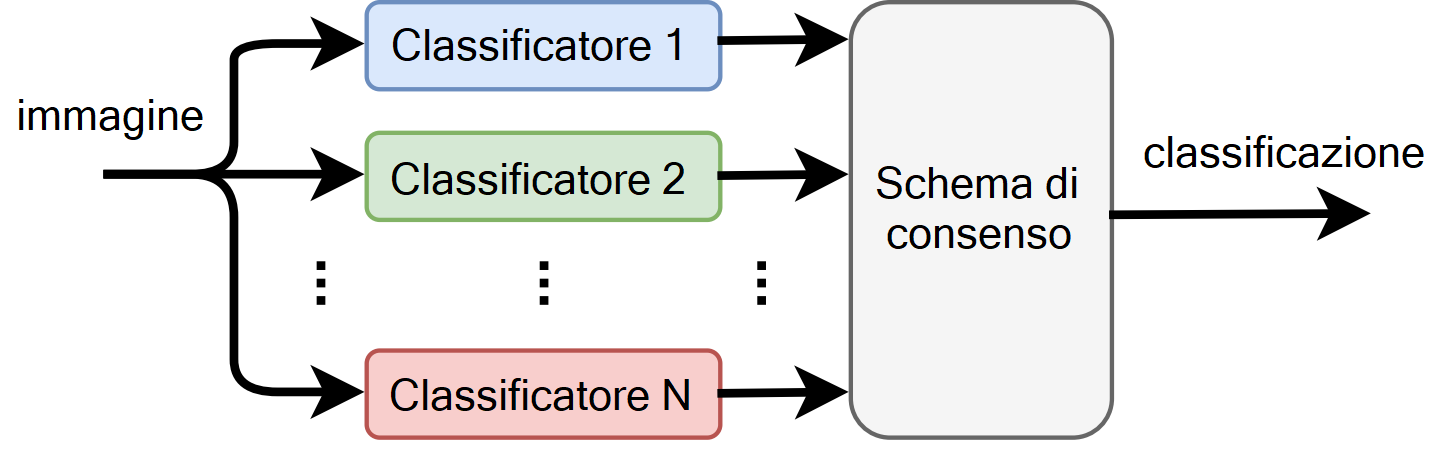
\includegraphics[width=0.9\textwidth]{ensembleSchema}
\caption{Schema di un classificatore ensemble}
\label{fig:ensembleSchema}
\end{figure}

Gli schemi di consenso più utilizzati sono i seguenti:

\begin{itemize}
\item \textbf{\textit{Hard major voting}} (HMV): la classe predetta per l'immagine in input è quella che ha ricevuto il maggior numero di "voti" (predizioni) da parte delle reti dell'ensemble.

\item \textbf{\textit{Soft major voting}} (SVM): la classe predetta per l'immagine in input è quella la cui probabilità di classificazione media (cioè la media delle probabilità softmax relative a quella classe attribuite dalle reti dell'ensemble) è la più grande.
\end{itemize}

L'efficacia dei metodi ensemble è dovuta al fatto che, solitamente, differenti modelli addestrati per risolvere uno stesso problema di classificazione non faranno tutti gli stessi errori sul \textit{test set} (gli errori si possono cioè considerare, in buona sostanza, incorrelati). Se lo schema di consenso applicato è il \textit{major voting}, si dimostra che l'ensemble di classificatori ha sempre prestazioni migliori o almeno uguali a quelle di ciascuna rete dell'ensemble presa singolarmente; il miglioramento delle prestazioni (specificamente della \textit{test accuracy}\footnote{training/validation/test accuracy = 1 -- training/validation/test error, par. \ref{overfitting}}) è tanto migliore quanto più gli errori commessi dalle reti dell'ensemble sono tra loro incorrelati.\cite{dlbook}\cite{ensembles}\\

Il nuovo classificatore per i ritagli delle pinne, oggetto di sviluppo in questo lavoro di tesi, è in realtà un \textit{ensemble} di tre reti neurali convoluzionali ri-addestrate con la tecnica del \textit{transfer learning} (par. \ref{esperimentoTL}).